\documentclass[12pt]{article}

\usepackage{sbc-template}
\usepackage{graphicx,url}
\usepackage[utf8]{inputenc}
\usepackage[brazil]{babel}
\usepackage{lipsum}
\usepackage{hyperref}
\usepackage{colortbl}
\usepackage{pgf, tikz}
\usepackage{multirow}
\usepackage[toc,page]{appendix}
\usepackage{afterpage}

\renewcommand{\tablename}{Tabela}
\renewcommand{\tableautorefname}{Tabela}

\renewcommand\appendixname{APÊNDICE}
\renewcommand\appendixpagename{APÊNDICE}

\addtolength{\intextsep}{-1pt}

\sloppy

\title{Desenvolvimento de uma Plataforma para a Gestão do Condomínio Madre Paulina}

\author{William S. Nepomuceno\inst{1}, Victor B. da Silva\inst{1}}

\address {
    Instituto de Tecnologia -- Universidade de Passo Fundo
    (UPF) \\
    Passo Fundo -- RS -- Brazil
    \email{178344@upf.br, victorbilly@upf.br}
}

\begin{document}

\maketitle

\begin{abstract}
This paper presents the proposal of a plataform for the management of the Madre Paulina condominium and also the development of improvements to the existing WEB platform. Initially it will describe the requirements and use cases raised with the end users, and it will also present the final result of the development, with images of the screens and explanation of the functioning. Finally, there will be an explanation of the technical implementation of the development, going through the Clean Architecture concepts and their layers, the SOLID Principles and the results obtained by applying the test-driven development.
\end{abstract}

\begin{resumo}
O presente trabalho apresenta a proposta de uma plataforma para a gestão do condomínio Madre Paulina e também o desenvolvimento de melhorias para a plataforma WEB já existente. Inicialmente será descrito os requisitos e casos de usos levantados com os usuários finais, passando pela apresentação das funcionalidades desenvolvidas para o aplicativo e a plataforma WEB. Por fim, terá uma explicação sobre a implementação técnica do desenvolvimento, passando pelos conceitos Clean Architeture e suas camadas, os Princípios SOLID e os resultados obtidos ao aplicar o desenvolvimento orientado a testes.
\end{resumo}

\section{Introdução e Contextualização}
Este projeto tem como objetivo o desenvolvimento de uma plataforma para a gestão do condomínio Madre Paulina, localizado em Tapejara - Rio Grande do Sul.

Atualmente o condomínio Madre Paulina conta com quinze condôminos, sendo duas salas comerciais, devido a quantidade de condôminos, para facilitar a gestão das tarefas diárias, o condominío possui uma plataforma WEB para o gerenciamento de suas atividades, desenvolvida pelo própio autor durante a disciplina de Laboratório de Engenharia de Software em 2022/1.

O backend da plataforma WEB foi desenvolvido utilizando o framework Laravel \cite{laravel} e o frontend utilizando o framework Angular \cite{angular}, que se comunicam através de uma API Rest.
Os serviços de Backend e Frontend estão hospedados no Heroku \cite{appMadrePaulinaWeb}, que é uma plataforma de hospedagem de serviços web. Para o banco de dados foi utilizado o SGBD MySQL \cite{mysql}, atualmente hospedado nos serviços RDS da Amazon Web Services \cite{amazonrds}.

O aplicativo foi desenvolvido utilizando a linguagem de programação Dart \cite{dart} e o framework Flutter \cite{flutter}, que permite o desenvolvimento de aplicações móveis para os sistemas operacionais Android e iOS, o aplicativo também irá se comunicar com o backend através de uma API Rest. O aplicativo está disponível para download na Play Store \cite{appMadrePaulina}.

\subsection{Motivação}
A partir do cenário atual do condomínio Madre Paulina, aliado com o crescimento da demanda contábil sobre a administração de condomínios onde é cada vez mais necessário obter informações precisas para a tomada de decisão, a fim de evitar um déficit nas contas, e levando em consideração que neste condomínio ainda são realizados de forma manual em cadernos, causando transtornos na prestação de contas, pela perda de informações, urge a necessidade de uma ferramenta que possibilite e facilite a contabilidade do condomínio Madre Paulina de forma mais precisa.

\subsection{Limitação}
Devido ao alto custo para a publicação de uma versão do aplicativo para o sistema operacional iOS, a publicação do aplicativo estará limitada somente à plataforma Android.
Devido ao curto prazo para o desenvolvimento, não foram realizadas avaliações de experiência com os usuários referentes a usabilidade e possíveis melhorarias para a plataforma WEB e do aplicativo móvel.

\section{Modelagem da aplicação}
Na base da modelagem dos projetos estão os seus requisitos, é fundamental que ao se desenvolver um sistema saibamos quais as necessidades das partes interessadas: usuários, clientes, fornecedores, desenvolvedores, empresas e o que o sistema deverá fazer para satisfazer essas necessidades.

Também é importante ponderar que os requisitos da aplicação disponibilzaram a base para o planejamento do desenvolvimento aplicação, bem como critérios para testes.

\subsection{Requisitos do sistema}
Requisitos definem o que um sistema deve fazer e sob quais restrições. Requisitos relacionados com a primeira parte dessa definição — o que um sistema deve fazer, ou seja, suas funcionalidades, ou até mesmo o que um sistema não deve fazer — são chamados de Requisitos Funcionais. Já os requisitos relacionados com a segunda parte — sob que restrições — são chamados de Requisitos Não-Funcionais \cite[Capítulo 3.1]{engsoftware}.

Após o levamento dos requisitos com o usuário final da aplicação, foram identificados os seguintes Requisitos Funcionais [\ref{Req-func}] e Requisitos Não-Funcionais [\ref{Req-nfunc}].

\subsubsection{Requisitos Funcionais}
\label{Req-func}
Nesta seção serão descritos os dois principais requisitos funcionais solicitados pelo usuário final.

\begin{center}
\begin{tabular}{| p{0.18\textwidth} | p{0.75\textwidth} |}
  \hline
  RF-001 & Adicionar usuário \\
  \hline
  RF-002 & Editar usuário \\
  \hline
  RF-003 & Adicionar período de Receitas / Despesas\\
  \hline
  RF-004 & Adicionar receita/despesa em um período \\
  \hline
  RF-005 & Remover receita/despesa de um período \\
  \hline  
   RF-006 & Relatório do Fluxo de Caixa \\
  \hline
   RF-007 & Cadastrar Condomínio \\
  \hline  
  RF-008 & Cadastrar Condômino \\
  \hline 
  RF-009 & Informar leitura d’água \\
  \hline
\end{tabular}
\end{center}

Inicialmente estava previsto também o desenvolvimento de outras duas funcionalidades, sendo a Reversa do Salão de Festas e Atas de Assembleia, porém os usuários finais não chegaram em um conceso quanto as regras de negócios.

Outras funcionalidades, como a Integração com o Internet Baking para a geração dos boletos do condominío, não foram desenvolvidas por falta de tempo.

\subsubsection{Requisitos Não-Funcionais}
\label{Req-nfunc}
Nesta seção serão descritos os dois principais requisitos não-funcionais.

\begin{center}
\begin{tabular}{| p{0.18\textwidth} | p{0.75\textwidth} |}
  \hline
  \multicolumn{2}{|c|}{\cellcolor{gray!30}Segurança} \\
  \hline
  RNFSEG-001 & Apenas usuários cadastrados deverão ter acesso ao sistema, 
  por meio de login. \\
  \hline
  RNFSEG-002 & As requisições às apis deverão ser autenticadas por meio de Json Web Token. \\
  \hline
  RNFSEG-003 & As senhas dos usuários deverão estar criptografadas. \\
  \hline
  \multicolumn{2}{|c|}{\cellcolor{gray!30}Interface} \\
  \hline
  RFNINT-001 & O aplicativo deve ter uma interface visual de fácil compreensão. \\
  \hline
\end{tabular}
\end{center}

\subsection{Casos de usos}
Casos de uso são documentos textuais de especificação de requisitos. Um caso de uso enumera os passos que um ator (usuário) realiza em um sistema com um determinado objetivo. Um caso de uso inclui duas listas de passos, sendo a primeira o fluxo normal, que são os passos necessários para concluir uma operação com sucesso. A segunda representa extensões desse fluxo normal, geralmente casos de exeções \cite[Capítulo 3.1]{engsoftware}. A \autoref{fig:UC_Diagram} apresenta o Diagrama de Casos de Usos.

\begin{figure}[!ht]
  \centering
  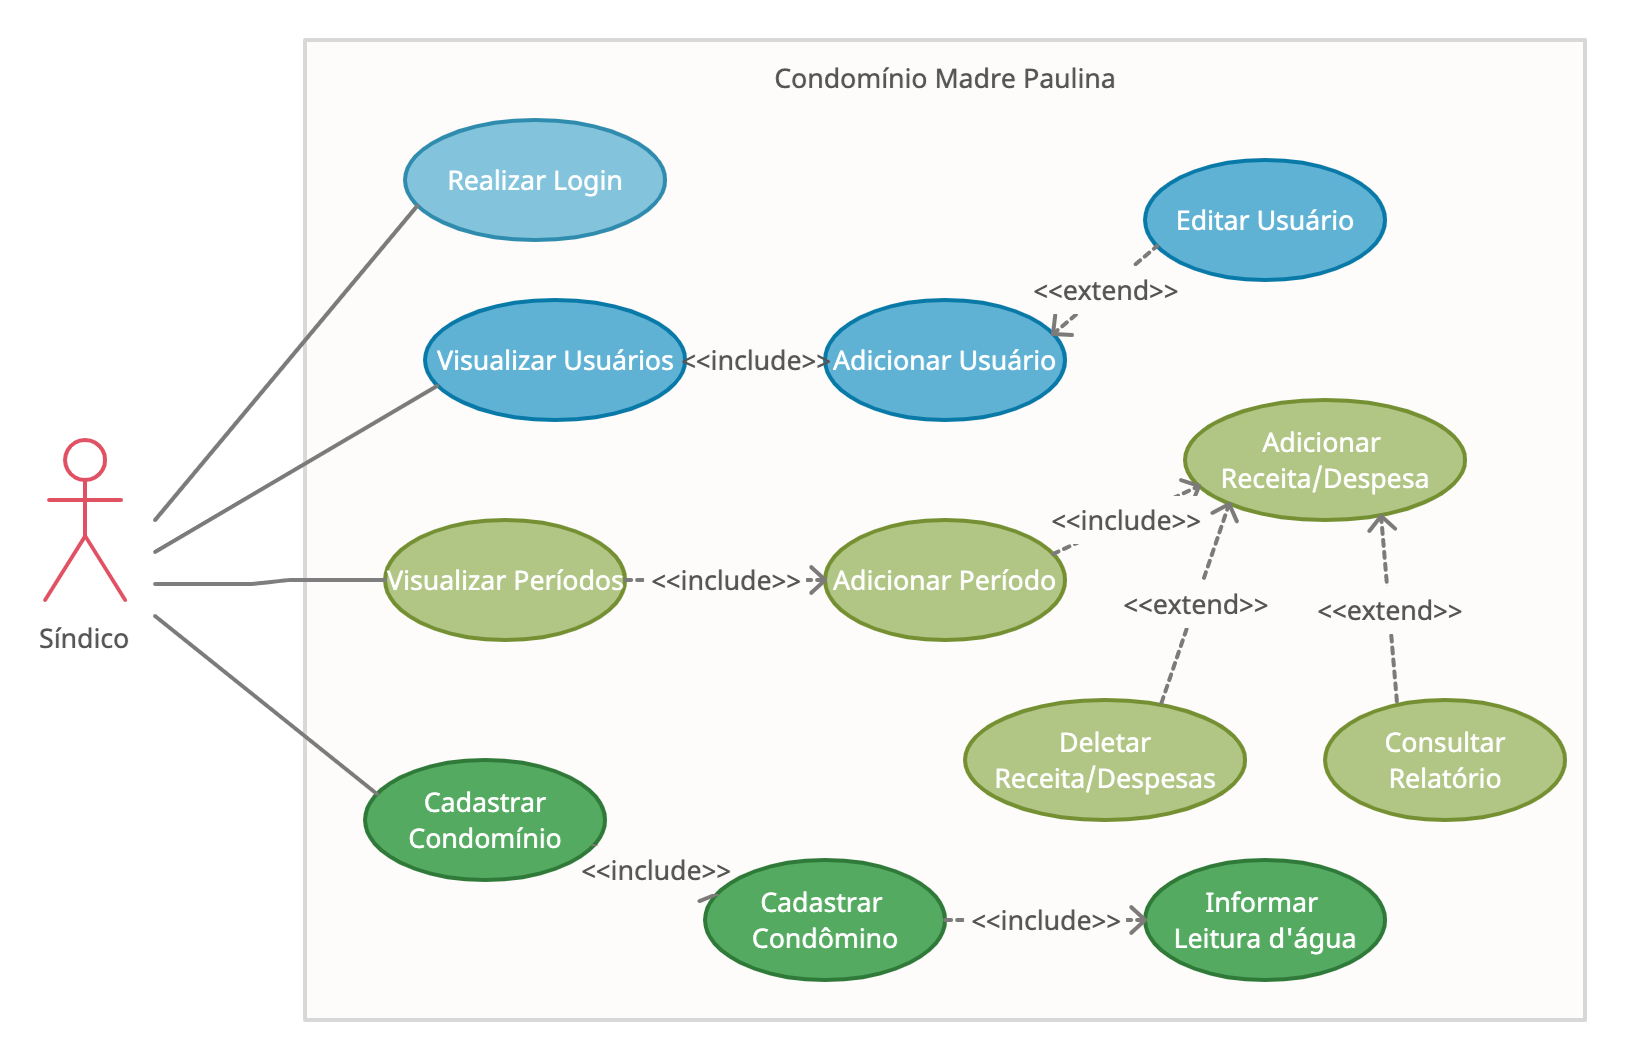
\includegraphics[width=0.8\columnwidth]{projeto/images/UC_Diagram.png}
  \caption{Diagrama Casos de Usos}
  \label{fig:UC_Diagram}
\end{figure}

\section{Especificação dos Casos de Usos}
\label{sec:usecase_espec}
A especificação dos casos de usos de uma sistema é um documento funcional, que descreve as funcionalidade que o sistema deve ter, também é apresetando com o sistema deve reagir ao conjunto de dados de entrada que recebe, qual o processamento destes dados e qual a retorno esperado. Dentre os casos de uso do sistema apresentados no diagrama de casos de uso, foram escolhidos alguns para serem detalhados, nas seções abaixo.

\subsection{RF001 - Adicionar período de Receitas / Despesas}
\label{sec:rf001}
O usuário na condição de síndico, deve ter a possibilidade de adicionar um novo período. O cadastro deste período deve ser realizado por meio de um formulário, o usuário deve informar um Nome, Data Ínicio, Data fim e Status (Aberto / Fechado). Após a submissão os dados devem ser validados e se tudo estiver correto, então o período deve ser cadastrado e o usuário deve ser redirecionado para a tela de listagem de períodos. Por outro lado, caso os dados informados estejam incorretos, o aplicativo deve exibir uma mensagem de erro e não cadastrar o período.

\subsection{RF002 - Adicionar Usuário}
O usuário na condição de síndico, deve ter a possibilidade de adicionar um novo usuário. O cadastro desse usuário deve ser por meio de um formulário, o síndico deve informar um Nome, E-mail, Senha, Confirmação de Senha e Perfil. Após a submissão os dados devem ser validados e se tudo estiver correto, então o novo usuário deve ser cadastrado e o usuário deve ser redirecionado para a tela de listagem de usuários. Por outro lado, caso os dados informados estejam incorretos, o aplicativo deve exibir uma mensagem de erro e não cadastrar o novo usuário.

\subsection{RF-004 Adicionar receita/despesa}
\label{sec:add_rec_desp}
O usuário na condição de síndico, deve ter a possibilidade de adicionar uma nova receita/despesa (lançamentos) em um período.
Com um período cadastrado, deve ser possível adicionar uma nova receita/despesa para o respectivo período, esse cadastro deve ser realizado por meio de um formulário, onde devem ser informados uma Descrição, Valor, Data e Tipo (Entrada / Saída). Após a submissão os dados devem ser validados e se tudo estiver correto, então a receita/despesa deve ser adicionada ao período e o síndico deve ser redirecionado para a tela de detalhes do período.
Por outro lado, caso os dados informados estejam incorretos, o aplicativo deve exibir uma mensagem de erro e não adicionar a receita/despesa.

O aplicativo também não deve permitir adicionar uma receita/despesa ao período, caso ele esteja com o status \emph{Fechado} e então exibir uma mensagem de alerta e não adicionar a receita/despesa. O mesmo deverá acontecer caso haja uma tentativa de exclusão de uma Receita/Despesa.

\subsection{RF-007 Cadastrar Condomínio}
O usuário na condição de síndico, deve ter a possibilidade de cadastrar os dados referentes ao seu condomínio. O cadastro deve ser feito realizado por meio de uma formulário, o síndico deve informar, Nome, CNPJ, Valor condomínio 2 quartos, Valor condomínio 3 quartos, Valor Condóminio Sala Comercial, Valor m³ d'água, Taxa de uso sala de festas, Taxa limpeza salão de festas, Taxa de mudança. Após a submissão os dados devem ser validados e se tudo estiver correto, então o condomínio deve ser cadastrado e o síndico deve ser redirecionado para a tela de listagem de condomíninos. Por outro lado, caso os dados informados estejam incorretos, o sistema deve exibir uma mensagem de erro e não cadastrar condomínino. 
A aplicação também deverá possuir um histórico de valores, pois todo ano há reajustes nos valores cobrados pelo condomínio.

\subsection{RF-008 Cadastrar Condômino}
O usuário na condição de síndico, deve ter a possibilidade de cadastrar os condôminos do seu condomínio. Com um Condomínio cadastrado, deve ser possível por meio de uma mestre detalhe, adicionar os moradores do condomínio. O síndico deve informar, Número do apartamento, Nome, CPF, Síndico [Sim/Não], Tipo [Apartamento, Sala Comercial], Número de quartos, Ativo [Sim / Não], Ordem. Após a subimissão os dados devem ser validados e se tudo estiver correto, então o condômino deve ser cadastrado, caso contrário o sistema deve exibir uma mensagem de erro e não cadastrar o condômino.

\section{Desenvolvimento da Aplicação}
A partir da Especificação dos Casos de Usos, foi possível dar início ao desenvolvimento da aplicação, o desenvolvimento ficou divido em duas plataformas, sendo elas um Aplicativo Móvel [\ref{sec:app_mobile}] e uma Plataforma WEB [\ref{sec:plataforma_web}].

\subsection{Aplicativo Móvel}
\label{sec:app_mobile}
Dentre as funcionalidades desenvolvidas para o aplicativo móvel está a interface para a implementação do caso de uso Adicionar Período [\ref{sec:rf001}].
A partir do cadastro de um novo período, conforme a Figura \ref{fig:UI_add_period}, é possível iniciar o lançamento de Receitas e Despesas conforme o caso de uso Adicionar receita/despesa [\ref{sec:add_rec_desp}], para adicionar um lançamento é necessário informar uma Descrição, Valor, Data e Tipo, conforme Figura \ref{fig:UI_add_period_details}.

\begin{table*}[!ht]
    \begin{minipage}{.4\linewidth}
        \centering
        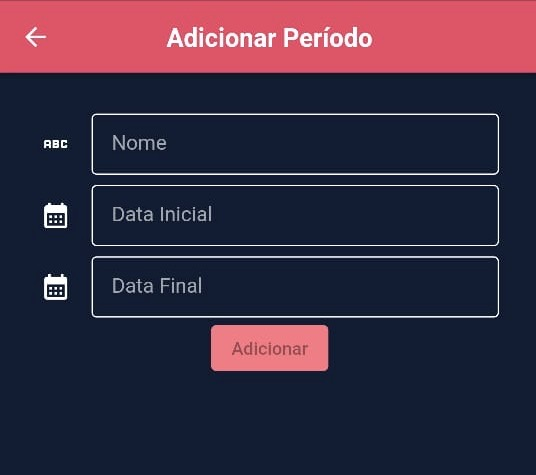
\includegraphics[width=0.9\columnwidth]{projeto/images/UI_add_period.jpeg}
        \captionof{figure}{Cadastro de período}
        \label{fig:UI_add_period}
    \end{minipage}
    \hfill
    \begin{minipage}{.4\linewidth}
        \centering
        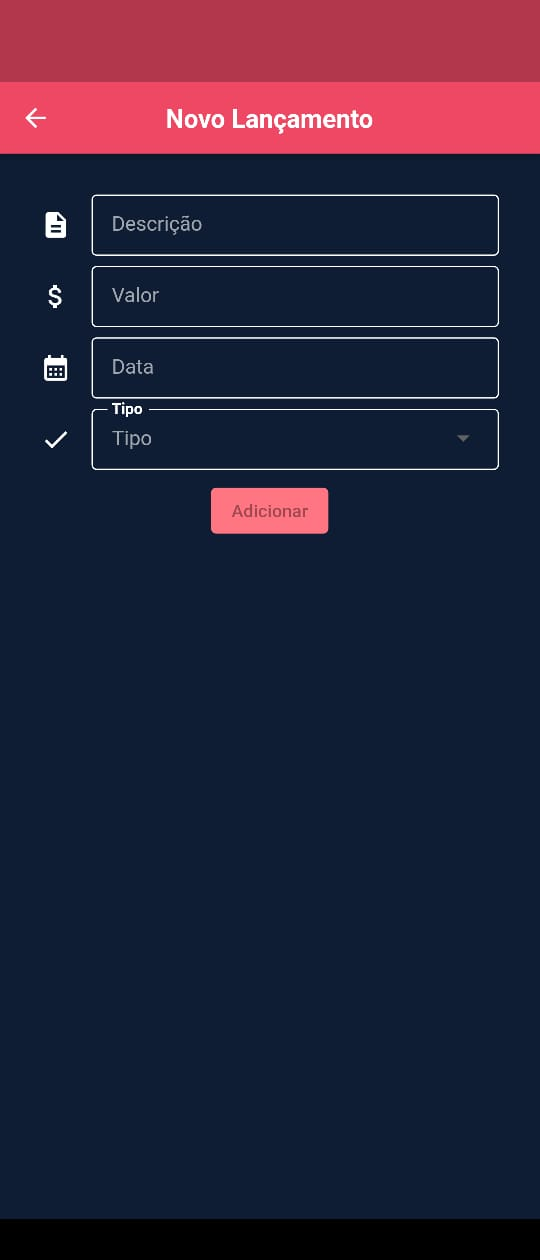
\includegraphics[width=0.9\columnwidth]{projeto/images/UI_add_period_details.jpeg}
        \captionof{figure}{Cadastro de receita/despesa}
        \label{fig:UI_add_period_details}
    \end{minipage}
\end{table*}

O aplicativo também dispõe de uma tela para que o Síndico possa acompanhar o resumo mensal do condomínio, conforme Figura \ref{fig:UI_Period_Details}, a tela  exibe o montante de entrada e de saída e o respectivo saldo para o respectivo período, esta tela também fornece o histórico de lançamentos para o período.

Outra funconalidade implementada nesta tela, é a validação para bloquear a adição ou exclusão de um lançamento do período,caso ele esteja com o status \emph{Fechado}, conforme a especificação do caso de uso Adicionar receita/despesa [\ref{sec:add_rec_desp}], a Figura \ref{fig:UI_Delete_Period_Details} mostra o resultado da implementação deste caso de uso.

\begin{table*}[!ht]
    \begin{minipage}{.4\linewidth}
        \centering
        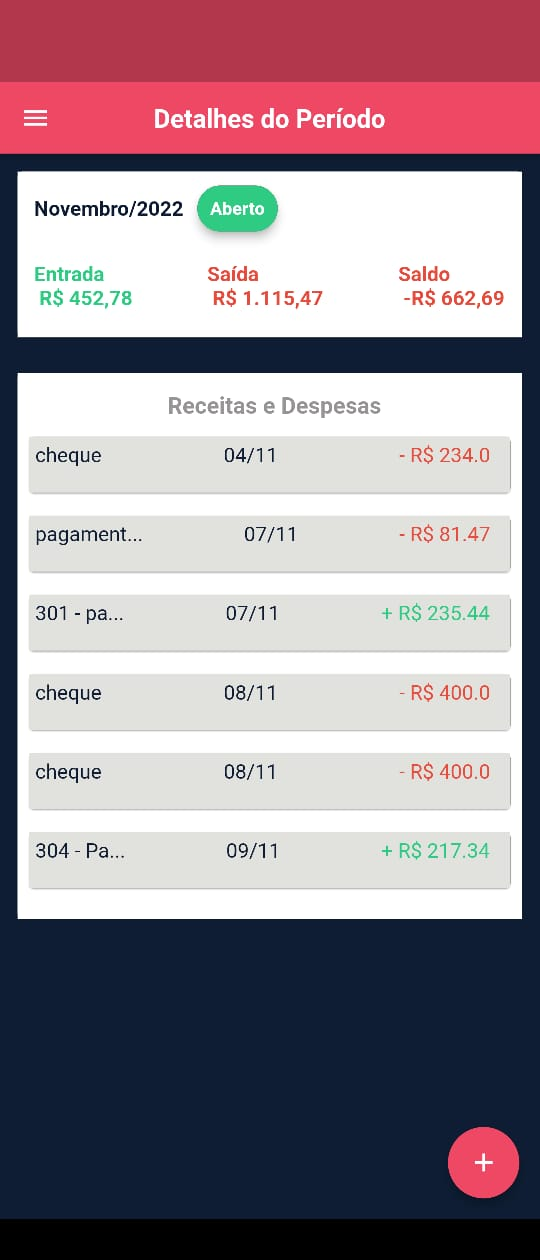
\includegraphics[width=0.8\columnwidth]{projeto/images/UI_Period_Details.jpeg}
        \captionof{figure}{Detalhes de um período}
        \label{fig:UI_Period_Details}
    \end{minipage}
    \hfill
    \begin{minipage}{.4\linewidth}
        \centering
        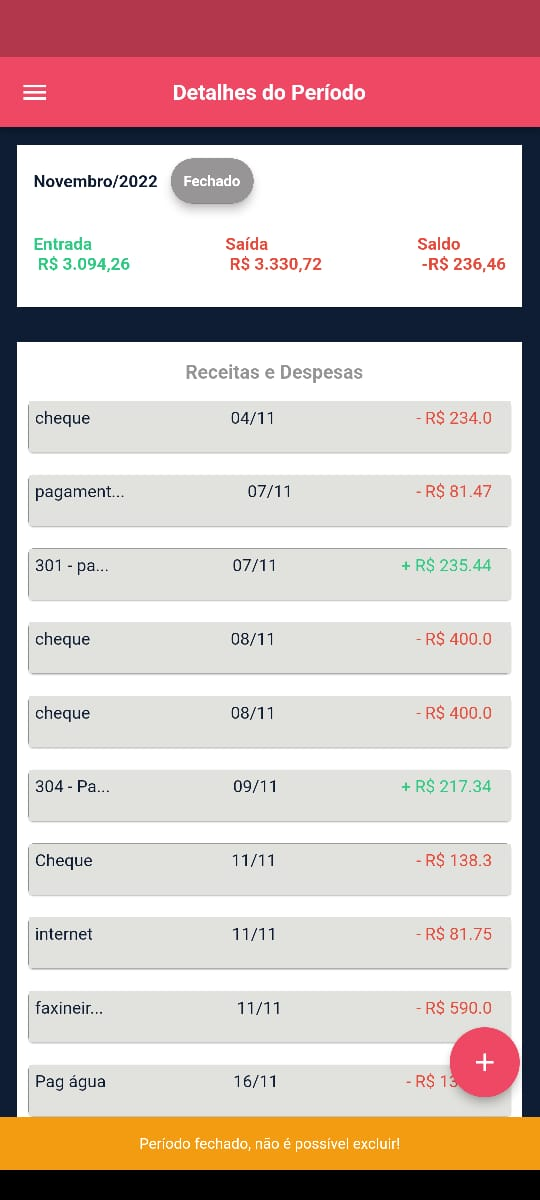
\includegraphics[width=0.8\columnwidth]{projeto/images/UI_Period_Details_Delete.jpeg}
        \captionof{figure}{Exclusão de um Detalhe do Perído}
        \label{fig:UI_Delete_Period_Details}
    \end{minipage}
\end{table*}

\subsection{Plataforma Web}
\label{sec:plataforma_web}

A plataforma WEB permite ao síndico gerenciar o condomínio e seus respectivos condôminos, nele também é possível gerenciar os valores do condomínio, algumas taxas básicas, como uso do salão de festas, taxa de mudança e outros valores referentes ao m³ da água e valor para a geração do boleto, conforme a \autoref{fig:UI_condominio}.

\begin{figure}[!ht]
  \centering
  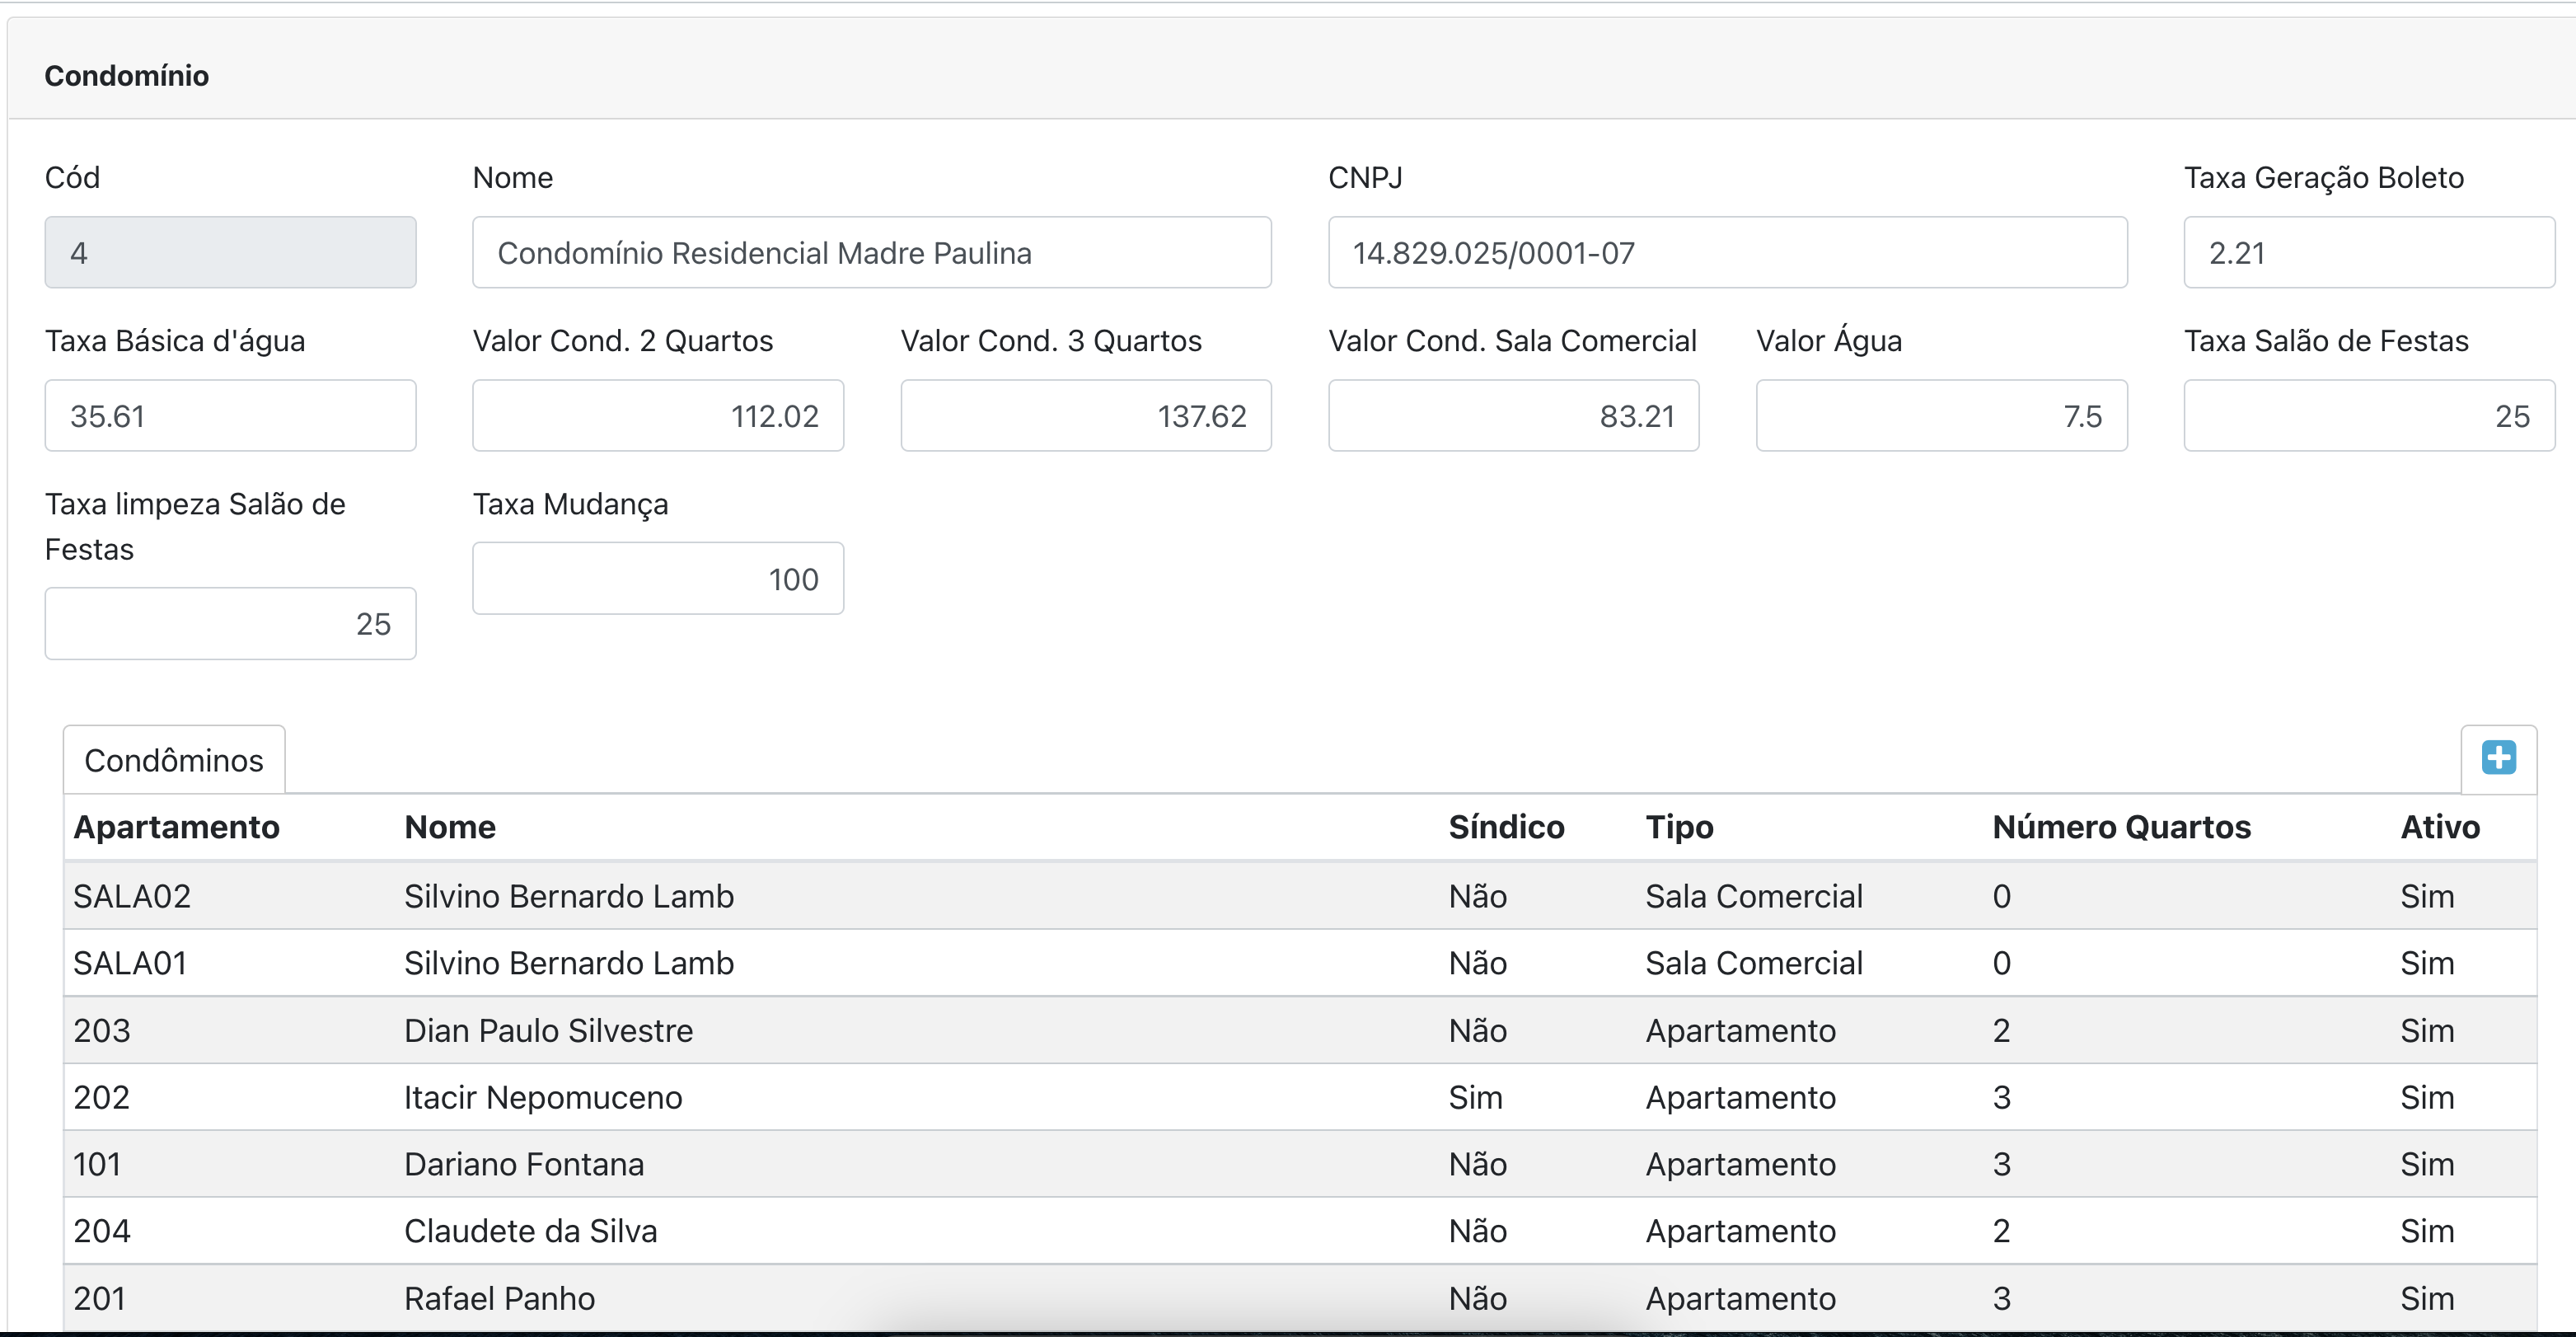
\includegraphics[width=0.8\columnwidth]{projeto/images/UI_condominio.png}
  \caption{Interface para manutenção do condomínio e condôminos}
  \label{fig:UI_condominio}
\end{figure}

Outra funcionalidade presente na plataforma, é a tela para realizar o gerencimaneto da leitura d’água de um período, \autoref{fig:UI_Geracaoagua}, sendo possível gerenciar o consumo d’água para cada apartamento, por meio de um cálculo automático, que considera o consumo feito na úlitma leitura e acrescidos dos valores referentes às taxas básicas, e se houverem, também podem ser adicionado os valores referentes às taxas de uso de salão de festas e mudanças. Após a geração dos boletos no Internet Banking é possível anexá-los, para que os condôminos possam visualizar os boletos por meio de um relatório.

\begin{figure}[!ht]
  \centering
  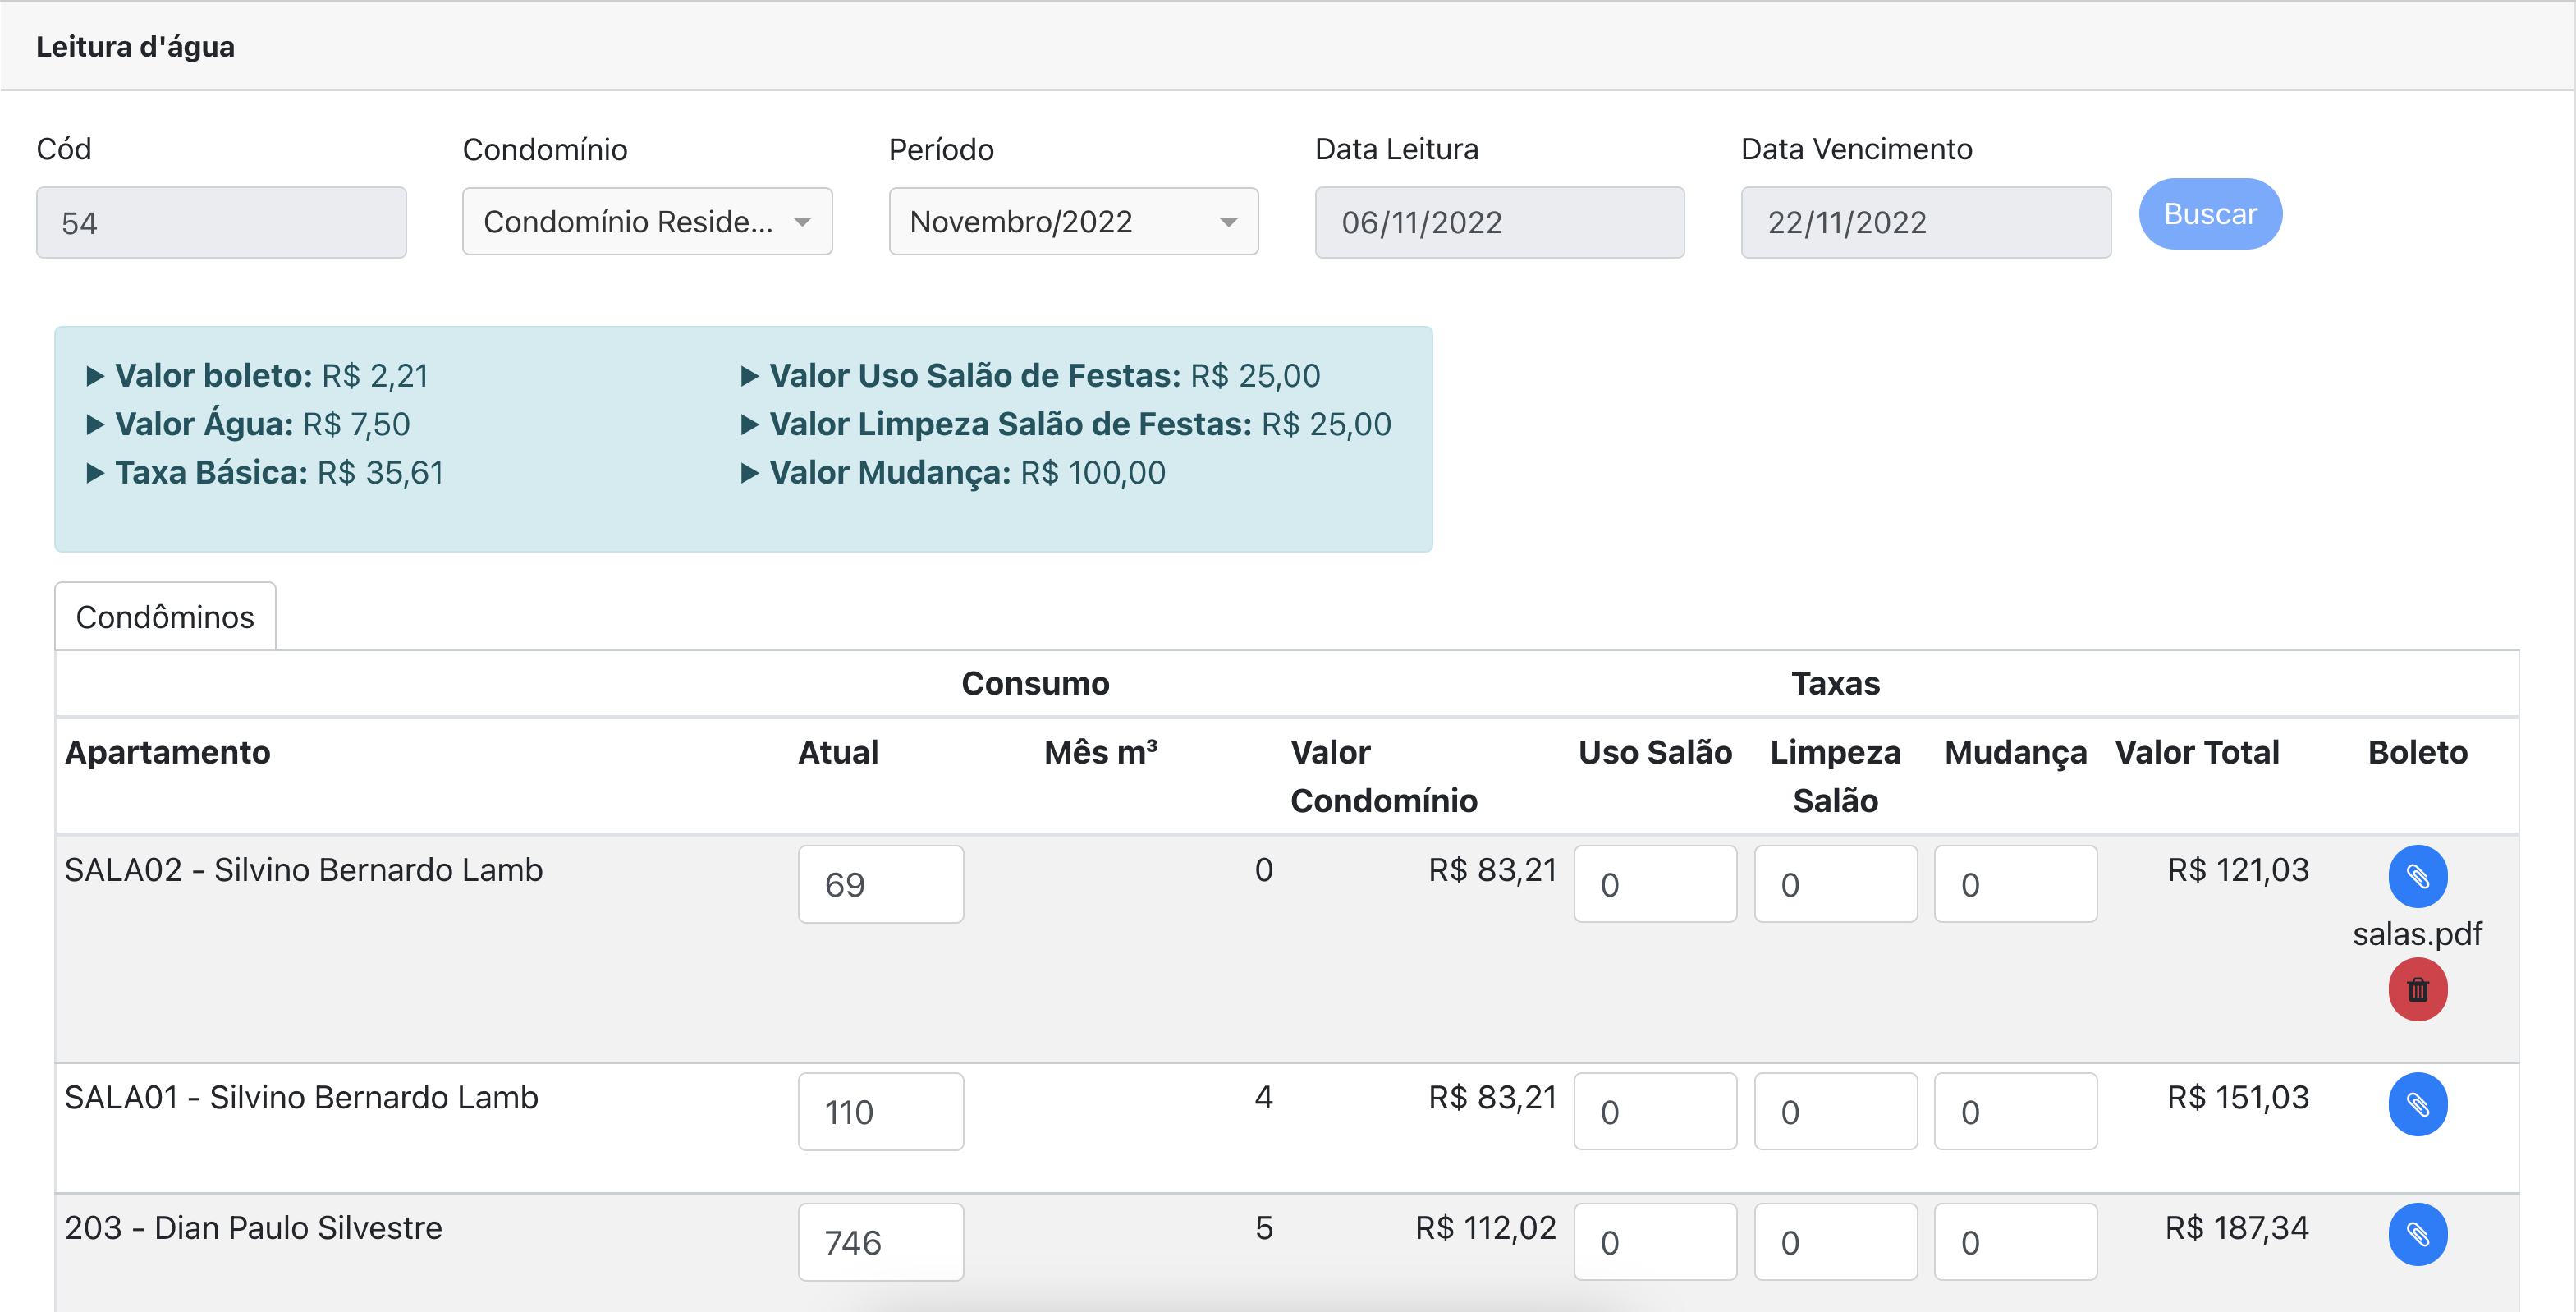
\includegraphics[width=0.8\columnwidth]{projeto/images/UI_Geracaoagua.png}
  \caption{Interface controle da leitura d`água}
  \label{fig:UI_Geracaoagua}
\end{figure}

A plataforma também dispõe um relatório, onde os condôminos podem acessar e acompanhar o seu consumo mensal d'àgua por meio de um gráfico de barras e também visualizar os boletos do condomínio, respectivamente \autoref{fig:UI_graph_consumo} e \autoref{fig:UI_report_consumo}. Neste relatório caso o usuário possua o perfil \emph{Condômino}, será exibido apenas os dados referentes ao seu apartamento, para usuários com o perfil de Síndico e Administrador, existe a possibilidade de aplicar um filtro por condômino.

\begin{figure}[!ht]
  \centering
  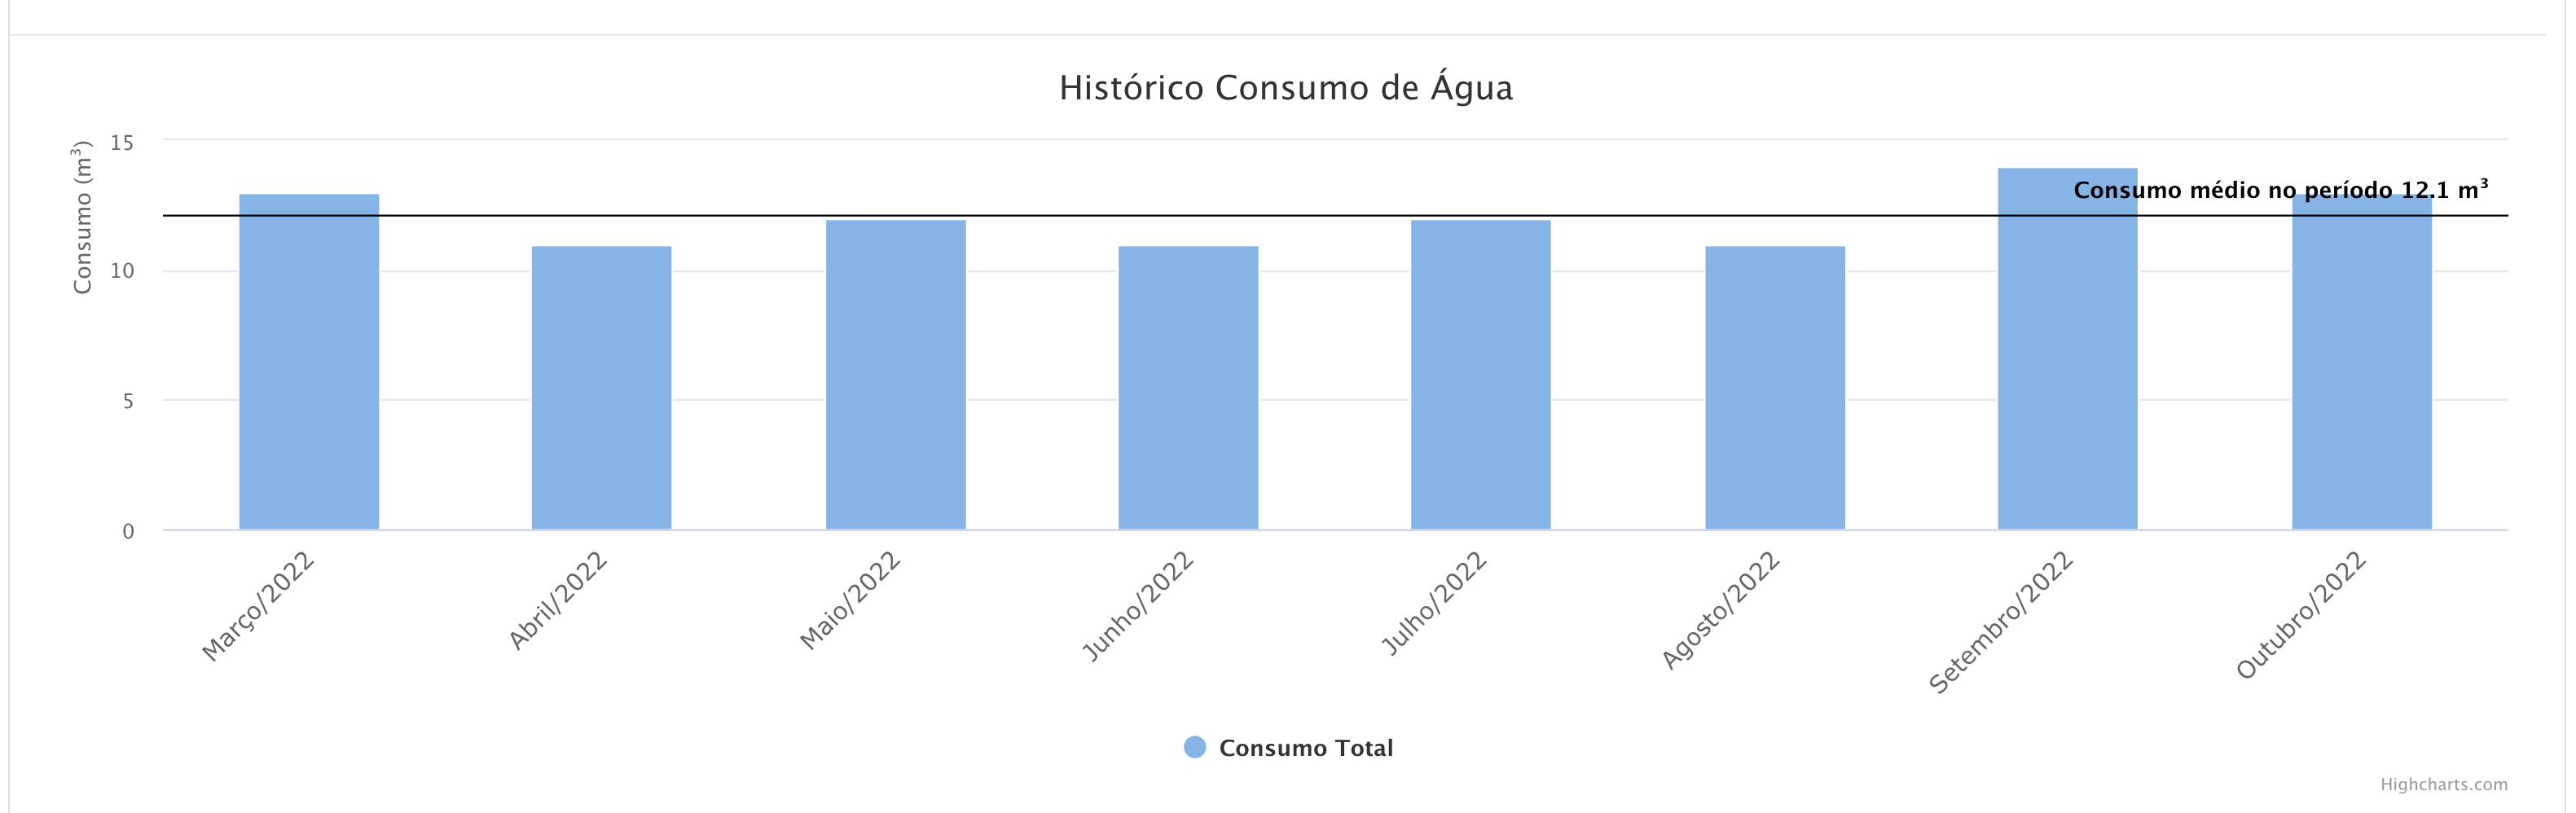
\includegraphics[width=0.8\columnwidth]{projeto/images/UI_graph_consumo.png}
  \caption{Gráfico consumo d`água}
  \label{fig:UI_graph_consumo}
\end{figure}

\begin{figure}[!ht]
  \centering
  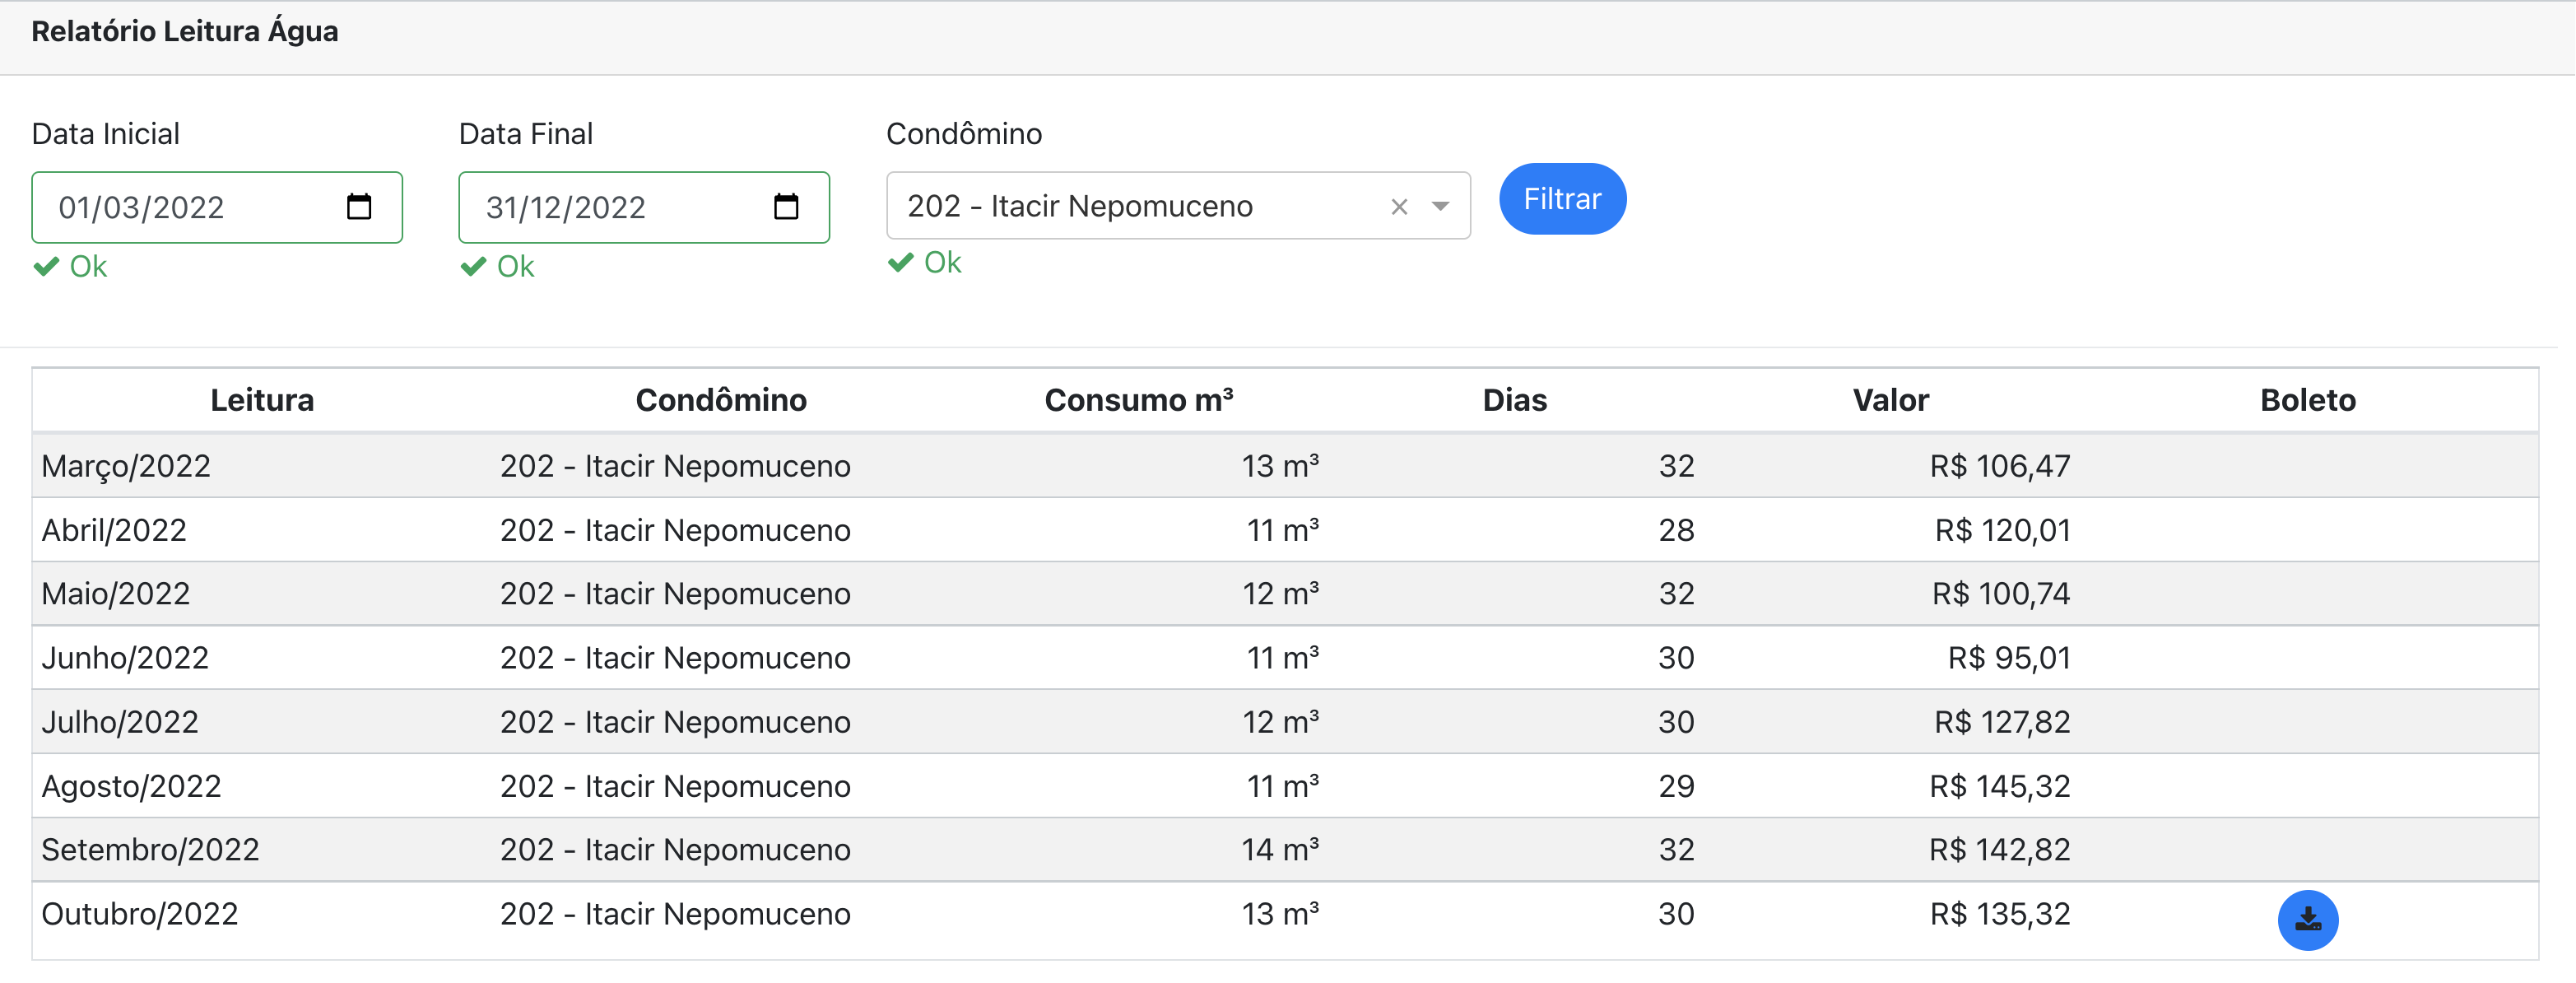
\includegraphics[width=0.8\columnwidth]{projeto/images/UI_report_consumo.png}
  \caption{Relatório leitura d`água}
  \label{fig:UI_report_consumo}
\end{figure}

Outro relatório administrativo que está presenta na plataforma é o de Relatório de Receitas e Despesas, \autoref{fig:UI_report_cashflow}. Neste relatório é possível visualizar as receitas/desepsas e o saldo mensal de um ano.
Na plataforma também estão disponíveis as funcionalidades referentes a cadastro de usuário e controle de permissões.

\begin{figure}[!ht]
  \centering
  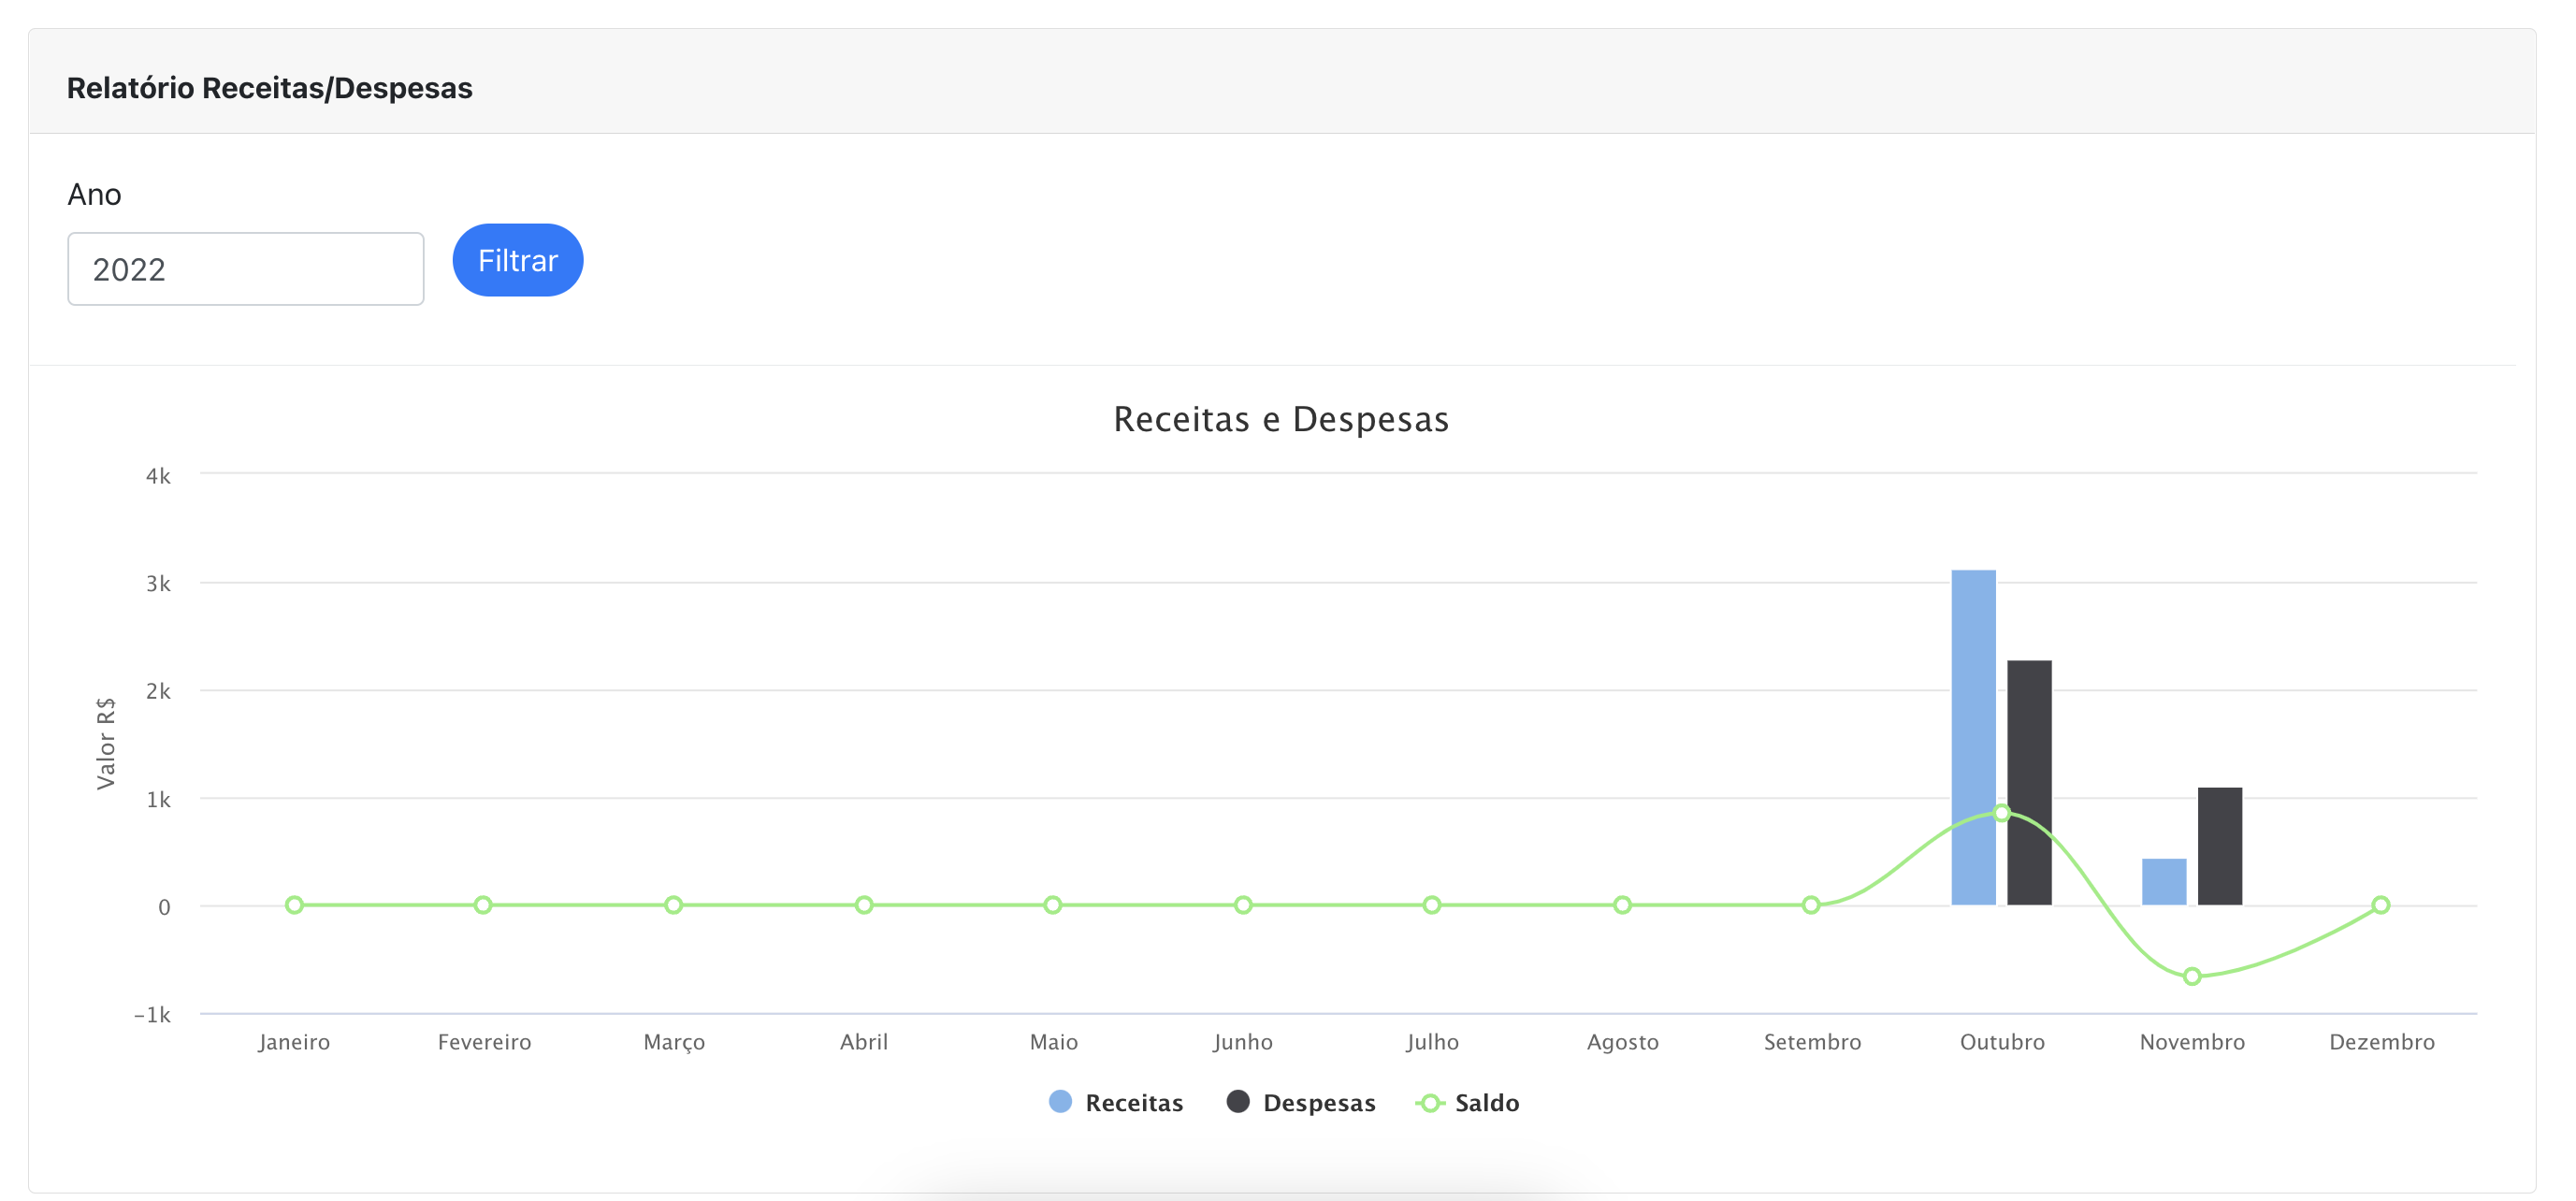
\includegraphics[width=0.8\columnwidth]{projeto/images/UI_report_cashflow.png}
  \caption{Relatório Receita/Despesas}
  \label{fig:UI_report_cashflow}
\end{figure}

\section{Implementação Técnica da Aplicação}
Para garantir uma boa qualidade de código, a aplicação foi desenvolvida seguindo os princípios do Test Driven Development [\ref{TDD}], que consiste em escrever os testes antes do código. Outro principio utilizado para desenvolvimento da aplicação foi o SOLID, que consiste em 5 princípios de orientação a objetos, que juntamente com os principíos de Clean Architecture, se seguidos garantem uma boa qualidade de código. As seções abaixo apresentam os detalhes destes principios aplicados ao projeto.

\subsection{Arquitetura}
Para o desenvolvimento da aplicação foi adotada arquitetura em camadas, que é um dos padrões arquiteturais mais usados, desde que os primeiros sistemas de software de maior porte foram construídos nas décadas de 60 e 70. Em sistemas que seguem esse padrão, as classes são organizadas em módulos de maior tamanho, chamados de camadas. As camadas são dispostas de forma hierárquica, como em um bolo. Assim, uma camada somente pode usar serviços — isto é, chamar métodos, instanciar objetos, estender classes, declarar parâmetros, lançar exceções, etc. — da camada imediatamente inferior \cite[Capítulo 7.2]{engsoftware}. 

Conjuntamente com a arquitetura em camadas, foram aplicados os conceitos de Clean Architecture, conceitos estes definidos por Robert C. Martin em seu livro Clean Architecture: A Craftsman's Guide to Software Structure and Design, publicado em 2017 \cite{cleanArchitecture}.

\subsection{Clean Architecture (Arquitetura Limpa)}
Clean Architecture ou também chamada de Arquitetura Limpa é um padrão de projeto de software para arquitetura de software que segue os conceitos de código limpo e implementa princípios SOLID [\ref{SOLID}].

Os padrões de projeto podem ser definidos como boas práticas que ajudam a manter a lógica de negócios unida para minimizar as dependências dentro do sistema. Seguindo a arquitetura limpa permite aos arquitetos de software desacoplar componentes para que fiquem isolados o suficiente para serem duráveis e facilmente alterados sem refazer o sistema.

Dessa forma, seguindos estas boas práticas foi elaborada a proposta de arquitetura para o requisito RF001 - Adicionar um novo usuário [\ref{Req-func}], representada através de um diagrama na Figura \ref{fig:DiagramaArquitetura}, a arquitetura dos demais casos de uso seguirão a mesma ideia. Os detalhes de cada camada serão explanados na seção [\ref{layers}].

\begin{figure}[!ht]
  \centering
  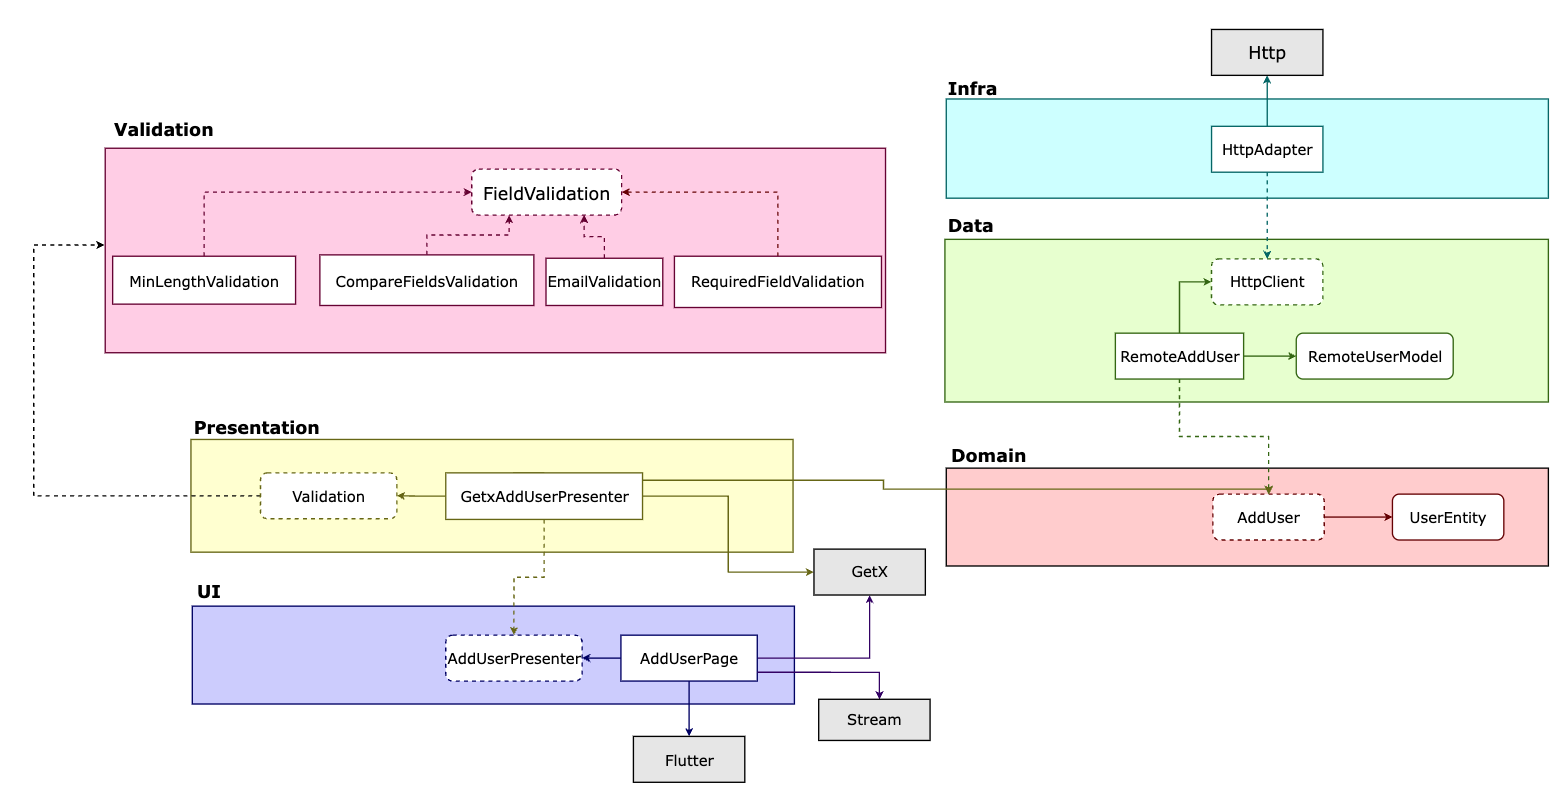
\includegraphics[width=\textwidth,height=\textheight,keepaspectratio]{projeto/images/DiagramaArquitetura.png}
  \caption{Proposta de Arquitetura para a aplicação.}
  \label{fig:DiagramaArquitetura}
\end{figure}

\subsection{Camadas}
\label{layers}
As camadas (layers) são o núcleo principal para arquitetura limpa. 
Para o desenvolvimento do aplicativo, foram utilizado sete camadas: Domínio, Dados, Infraestrutura, Principal, Apresentação, Interface de Usuário, Validação.

\subsubsection{Domain Layer (Camada de Domínio)}
\label{domainLayer}
A camada de domínio é uma abastração responsável por encapsular as regras de negócios do sistema e fornencer os casos de usos. Para manter essas classes simples, cada caso de uso deve ter responsabilidade apenas sobre uma única funcionalidadee não deve conter dados mutáveis. Em vez disso, os dados devem ser manipulados na camadas de dados [\ref{dataLayer}]. Utilizando a camada de domínio é possível obter alguns benefícios, entre eles, pemitir a divisão de responsanbilidade, reduzir a duplicação de código e melhorar a testabilidade do aplicativo.

\subsubsection{Data Layer (Camada de Dados)}
\label{dataLayer}
A camada de dados é responsável por acessar os dados de alguma fonte, seja ela um banco de dados, um arquivo, uma API, etc.
Esta camada implementa as regras de negócios definidas pela camada de domínio, ou seja, ela não deve conter nenhuma regra de negócio, apenas implementar as regras definidas pela camada de domínio.

\subsubsection{Infra Layer (Camada de Infraestrutura)}
\label{infraLayer}
Camada de infraestrutura é responsável por se comunicar com serviços externos, como por exemplo, um banco de dados, uma API, ou seja, qualquer serviço externo que a aplicação precise se comunicar, por meio de interfaces. Neste projeto a camada de infraestrtura é responsável por se comunicar com a API e também com a memória cache dos dispositivos.

\subsubsection{Main Layer (Camada Principal)}
\label{mainLayer}
A camada principal é responsável por realizar a composição das demais camadas, por meio de injeção de dependência \footnote{Injeção de dependência é uma técnica para livrar ou remover o acoplamento entre os objetos.}, sendo também responsável por inicializar a aplicação. Em casos de uma API, esta camada é responsável por inicializar o servidor web e expor as rotas da aplicação.

\subsubsection{Presentaion Layer (Camda de Apresentação)}
\label{presentantionLayer}
A camada de apresentação é responsável por expor a aplicação para o usuário, seja ela uma API, um site, um aplicativo, etc. Neste projeto, também é a camada responsável por executar as ações do usuário, como por exemplo, receber os dados de um formulário. 

Em casos de uma API, esta camada é responsável por receber os dados da requisição, realizar o processamento dos dados e dar um retorno para o usuário após o processamento.

\subsubsection{UI Layer (Camada de Interface de Usuário)}
\label{uiLayer}
A camada de interface de usuário é a camada onde o usuário interage com a aplicação. Neste projeto, a camada de interface é responsável por exibir os dados para o usuário, e também é responsável por receber as ações do usuário, como por exemplo um formulário, um botão, etc.

\subsubsection{Validation Layer (Camada de Validação)}
\label{validationLayer}
A camada de validação é responsável por realizar a validação de dados informados pelo usuário na camada UI. Para o projeto foi implementada a validação de tamanho mínimo de um campo, e-mail, CPF, senha e confirmação de senha.

\subsection{Princípios SOLID}
\label{SOLID}
Os princípios SOLID são cinco princípios de programação orientada a objetos e design de código que ajudam a tornar os códigos mais fáceis de entender, manter e estender \footnote{Exemplos e Aplicação dos conceitos SOLID estão descritos no \autoref{apx:solid}.}. Os princípios SOLID foram definidos por Robert C. Martin em seu livro Clean Architecture \cite{cleanArchitecture}, os 5 princípios que compõe o SOLID são:
 
% \subsubsection{S - Single Responsibility Principle (Princípio da Responsabilidade Única)}
% \label{SRP}
% O princípio da responsabilidade única (SRP) diz que uma classe deve ter apenas uma responsabilidade. Em outras palavras, uma classe deve ter apenas uma razão para mudar. Ao aplicarmos este princípio podemos obter alguns benefícios, como a facilidade na manutenção do código, facilidade para o desenvolvimento de testes e permite que os códigos sejam reutilizáveis.

% \subsubsection{O - Open/Closed Principle (Princípio Aberto/Fechado)}
% \label{OCP}
% O Princípio Aberto/Fechado (OCP) é um dos princípios mais importantes do SOLID. Ele diz que as classes devem estar abertas para extensão, mas fechadas para modificação. Ou seja, você deve ser capaz de estender o comportamento de uma classe sem precisar modificá-la.

\subsubsection{L - Liskov Substitution Principle (Princípio da Substituição de Liskov)}
\label{LSP}
O Princípio de Substituição de Liskov (LSP) diz que objetos podem ser substituídos por seus subtipos sem que isso afete a execução correta do programa. O principal objetivo do LSP é manter o funcionamento do código íntegro no processo de acoplamento de funcionalidades na aplicação. Esse princípio é quebrado em situações nas quais uma subclasse deixa de herdar um comportamento da classe pai, seja  sobrescrevendo um método e lançando uma exceção ou não tirando proveito  de todas as funcionalidades dela.

\subsubsection{I - Interface Segregation Principle (Princípio da Segregação da Interface)}
\label{ISP}
O Interface Segregation Principle (ISP) nos diz que uma classe não deve ser forçada a implementar uma interface que ela não irá utilizar. O ISP é um princípio que nos ajuda a manter nossas classes mais coesas e focadas em uma única responsabilidade. Um exemplo de ISP  é o uso de interfaces ou classes abstratas. Uma interface é um contrato que define um conjunto de métodos que uma classe deve implementar

\subsubsection{D - Dependency Inversion Principle (Princípio da Inversão da Dependência)}
\label{DIP}
O Dependency Inversion Principle (DIP) nos diz que os módulos de alto nível não devem depender de módulos de baixo nível. Ambos devem depender de abstrações e as abstrações não devem depender de detalhes. Um exemplo de DIP, assim como no ISP é o uso de interfaces, ou seja, uma classe pode depender de uma interface, mas não de uma implementação concreta.

\subsection{Test Driven Development}
\label{TDD}
Test Driven Development (TDD), ou Desenvolvimento Orientado a Testes, é uma prática de desenvolvimento de software sugerida por diversas metodologias ágeis, como o Extreme programming. A prática sugere aos desenvolvedores que os testes automatizados sejam escritos de maneira contínua, ao longo do desenvolvimento do software \footnote{Mais detalhes sobre os resultados obitos ao usar o TDD estão no \autoref{apx:tdd}}. Dessa forma a suíte de testes é maior, abrangindo mais cenários de testes \cite[Capítulo 8.1]{engsoftware}.

Para um melhor aproveitamento do uso do TDD, foram elaborados alguns casos de testes a nível de integração para a camada de dados do requisito funcional RF-003 Adicionar período de Receitas / Despesas [\ref{sec:add_rec_desp}], implementação \emph{RemotAddPeriod}, que faz uso da camada de infraestrutura para realizar as requisições para a API, usando a implementação da interface \emph{HttpClient}. Para isso, foram elaborados os seguintes casos de testes:

\begin{itemize}
    \item RemotAddPeriod deve chamar HttpClient com os valores corretos.
    \item RemotAddPeriod deve lançar UnexpectedError quando HttpClient retornar erro 400, 404, 500.
    \item RemotAddPeriod deve retornar um Period quando HttpClient retornar 200.
\end{itemize}

Na \autoref{fig:remote_add_period_test}, é possível analisar a implementação de um teste automatizado a nível de integração para a classe \emph{RemotAddPeriod}, nela inicialmente é criado um Spy \footnote{Spy é uma denominação dada a um objeto que grava suas interações com outros objetos.} para a classe HttpClient, este Spy irá armazenar os valores utilizados para realizar a requisição, além de permitir mockar erros, conforme podemos ver na \autoref{fig:httpClientSpy}. Posteriormente é realizado a chamada do metódo add do SUT (Sistema Sobre Testes) \footnote{Sistema Sobre Testes, refere-se a classe que está sendo testada.} e por fim é verificado se o metódo request do HttpClient foi chamado com os valores corretos.

\begin{figure}[!ht]
  \centering
  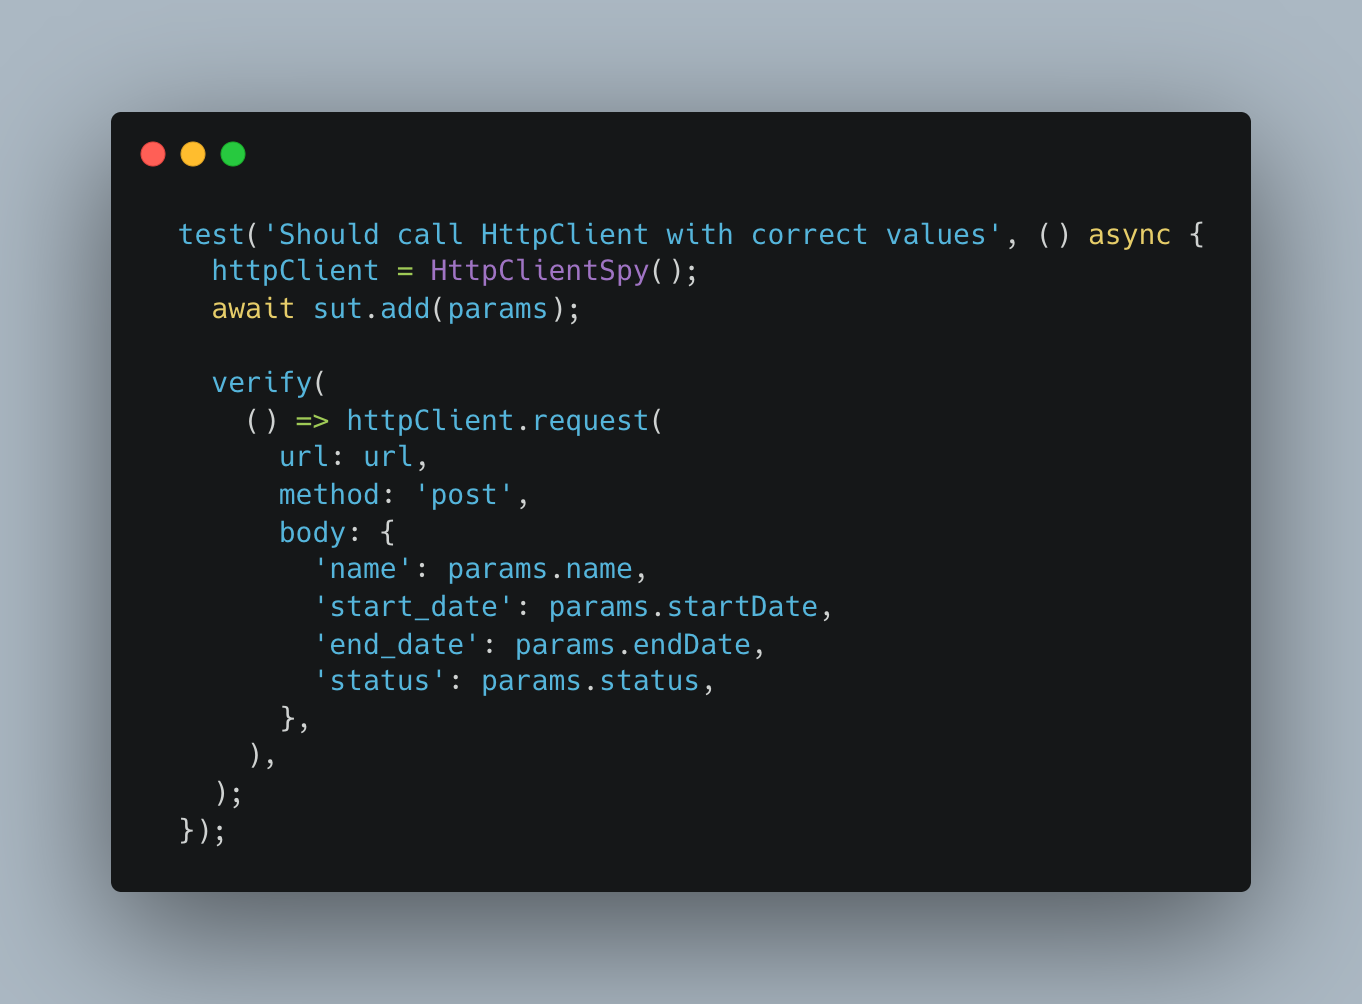
\includegraphics[width=0.9\columnwidth]{projeto/images/remote_add_period_test.png}
  \caption{Exemplo de um teste da classe RemoteAddPeriod}
  \label{fig:remote_add_period_test}
\end{figure}

Na figura \autoref{fig:remote_add_period_test_error} podemos ver um teste automatizado para verificar o retorno esperado para quando a implementação \emph{HttpClient} lançar uma exceção quando ocorrer um erro com o status http 500. Neste teste também é utilizada a classe HttpClientSpy, onde é feito um mock de erro do tipo \emph{ServeError} para a request.

Os testes para os demais casos de erros para os status 400 e 404, seguem o mesmo padrão, apenas mudando o tipo do erro utilizando no mock, sendo respectivamente \emph{BadRequest} e \emph{NotFound}.

\begin{figure}[!ht]
  \centering
  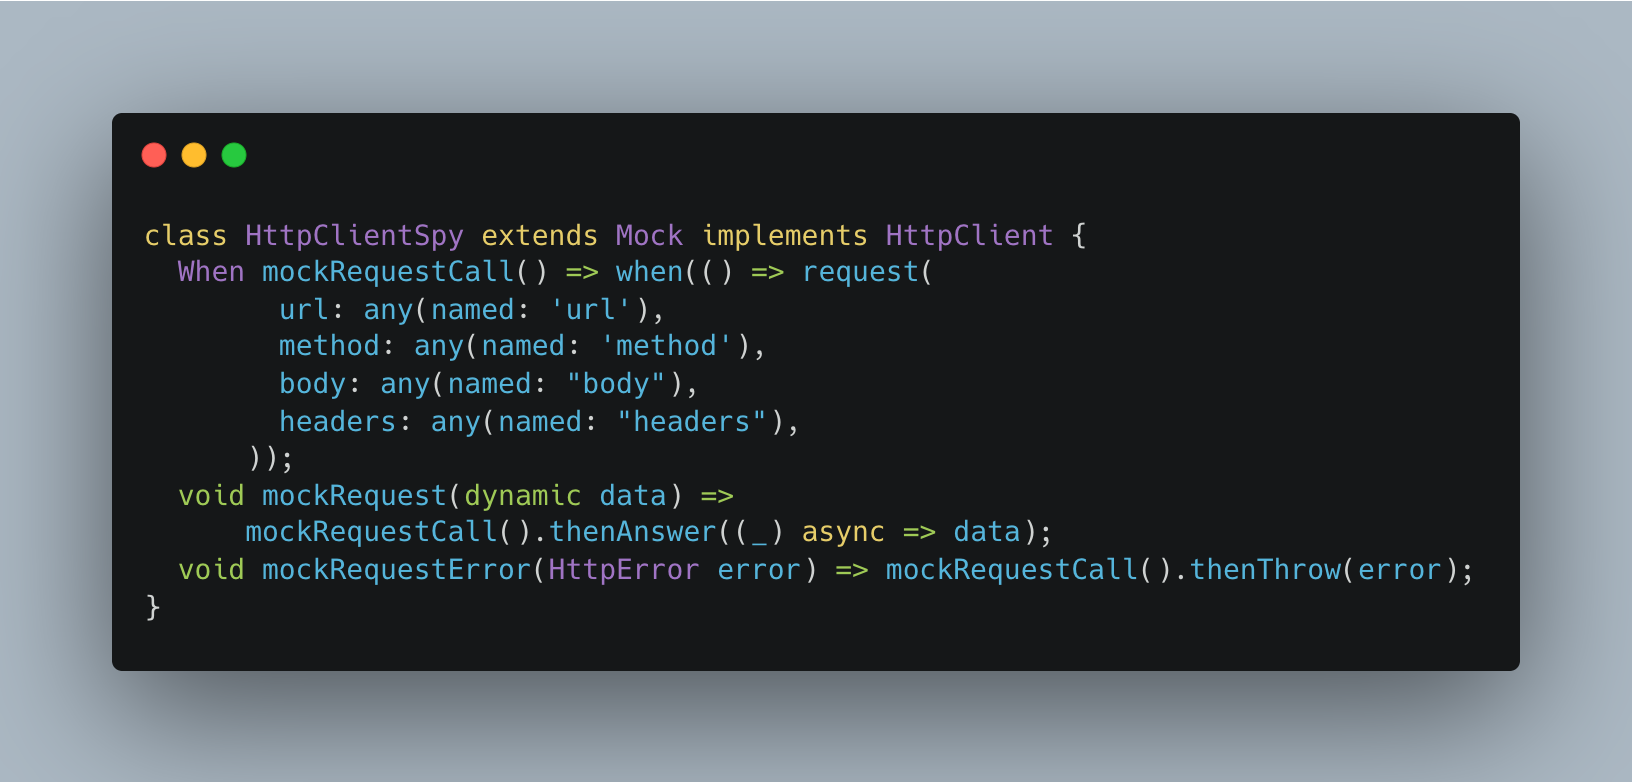
\includegraphics[width=0.9\linewidth]{projeto/images/http_client_spy_test.png}
  \caption{Spy para a classe Http Client}
  \label{fig:httpClientSpy}
\end{figure}

\begin{figure}[!ht]
  \centering
  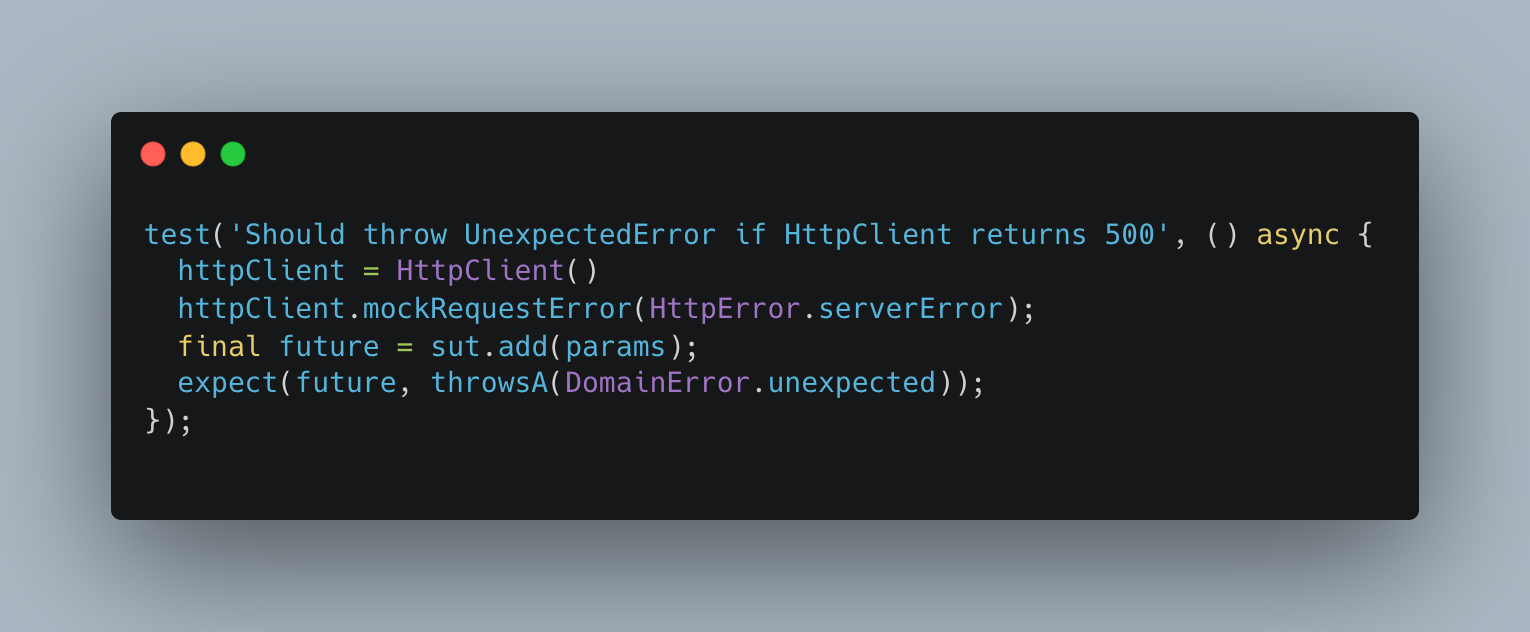
\includegraphics[width=0.9\columnwidth]{projeto/images/remote_add_period_test_error.png}
  \caption{Exemplo de um teste de erro da classe RemoteAddPeriod}
  \label{fig:remote_add_period_test_error}
\end{figure}

\section{Conclusões}
O presente projeto teve como objetivo o desenvolvimento de uma plataforma para o condomínio Madre Paulina. Durante o desenvolvimento procurou-se respeitar os requisitos funcionais e não-funcionais levantados com os usuários. Dessa o projeto abre caminho para que o condominío Madre Paulina e futuramente outros condominíos possam utilizar uma plataforma de análise e planejamento para melhorar tomadas de decisões, reduzindo custos, por exemplo.

Por outro lado, com o desenvolvimento orientado a testes, aliado aos princípios de Clean Architeture e SOLID, acredita-se que será possível adicionar novas funcionalidades para o aplicativo sem muito esforço. A aplicação destes conceitos e princípios também será de grande valia para a carreira profissional do autor, tendo em vista que o mercado da tecnologia da informação está cada vez mais exigente.

\section{Trabalhos Futuros}
Para o curto prazo, propõe-se realizar a entrega formal do aplicativo e das melhorias realizadas na plataforma ao condomínio Madre Paulina e realizar uma pesquisa com os usuários, a fim de avaliar a experiência durante o uso da aplicação, bem como elencar possíveis melhorias.

Outro ponto interessante para empreender um esforço, seria o de realizar um estudo sobre plataformas de hospedagem de serviços, considerando que a partir de novembro o Heroku não oferecerá mais serviços gratuitos. 

Por fim, sugere-se retomar com os usuários finais as funcionalidades referentes a Reversa do Salão de Festas e a Atas de Assembleia para definir as regras de negócio e posteriormente implementá-las. Também pode-se considerar o desenvolvimento da integração com o Internet Banking para a geração dos boletos, visto que atualmente a geração está sendo feita de forma manual, toranando-se uma atividade morosa.

\bibliographystyle{acm}
\bibliography{bibliography}

\newpage

\begin{appendices}
\section{Príncipios SOLID}
\label{apx:solid}
Neste apêndice estão alguns exemplos de aplicação dos princípios SOLID, utilizados durante o desenvolvimento da aplicação. 

\subsection{Princípio da Substituição de Liskov}
Neste projeto o LSP foi utilizado para sobrescrever as funcionalidades da classe \emph{HttpAdapter}, para que fosse possível realizar requisições HTTP autenticadas, ambas as classes implementam a interface \emph{HttpClient}. Essa sobrecarga foi feita utilizando o padrão de projeto Decorator, ou seja, é um padrão de projeto que nos permite adicionar novas funcionalidades  a um objeto dinamicamente, sem afetar o comportamento de outros objetos do mesmo tipo.

Conforme a \autoref{fig:lsp}, a classe \emph{AuthorizeHttpClientDecorator} implementa a interface HttpClient e também recebe um objeto do tipo HttpClient, chamado \emph{decoratee}, é este objeto que está sendo sobrescito. No metódo request podemos ver que está sendo adicionado um novo comportamento na classe e posteriormente repassando a ação para a classe pai, neste caso é a classe HttpAdapter.

\begin{figure}[!ht]
  \centering
  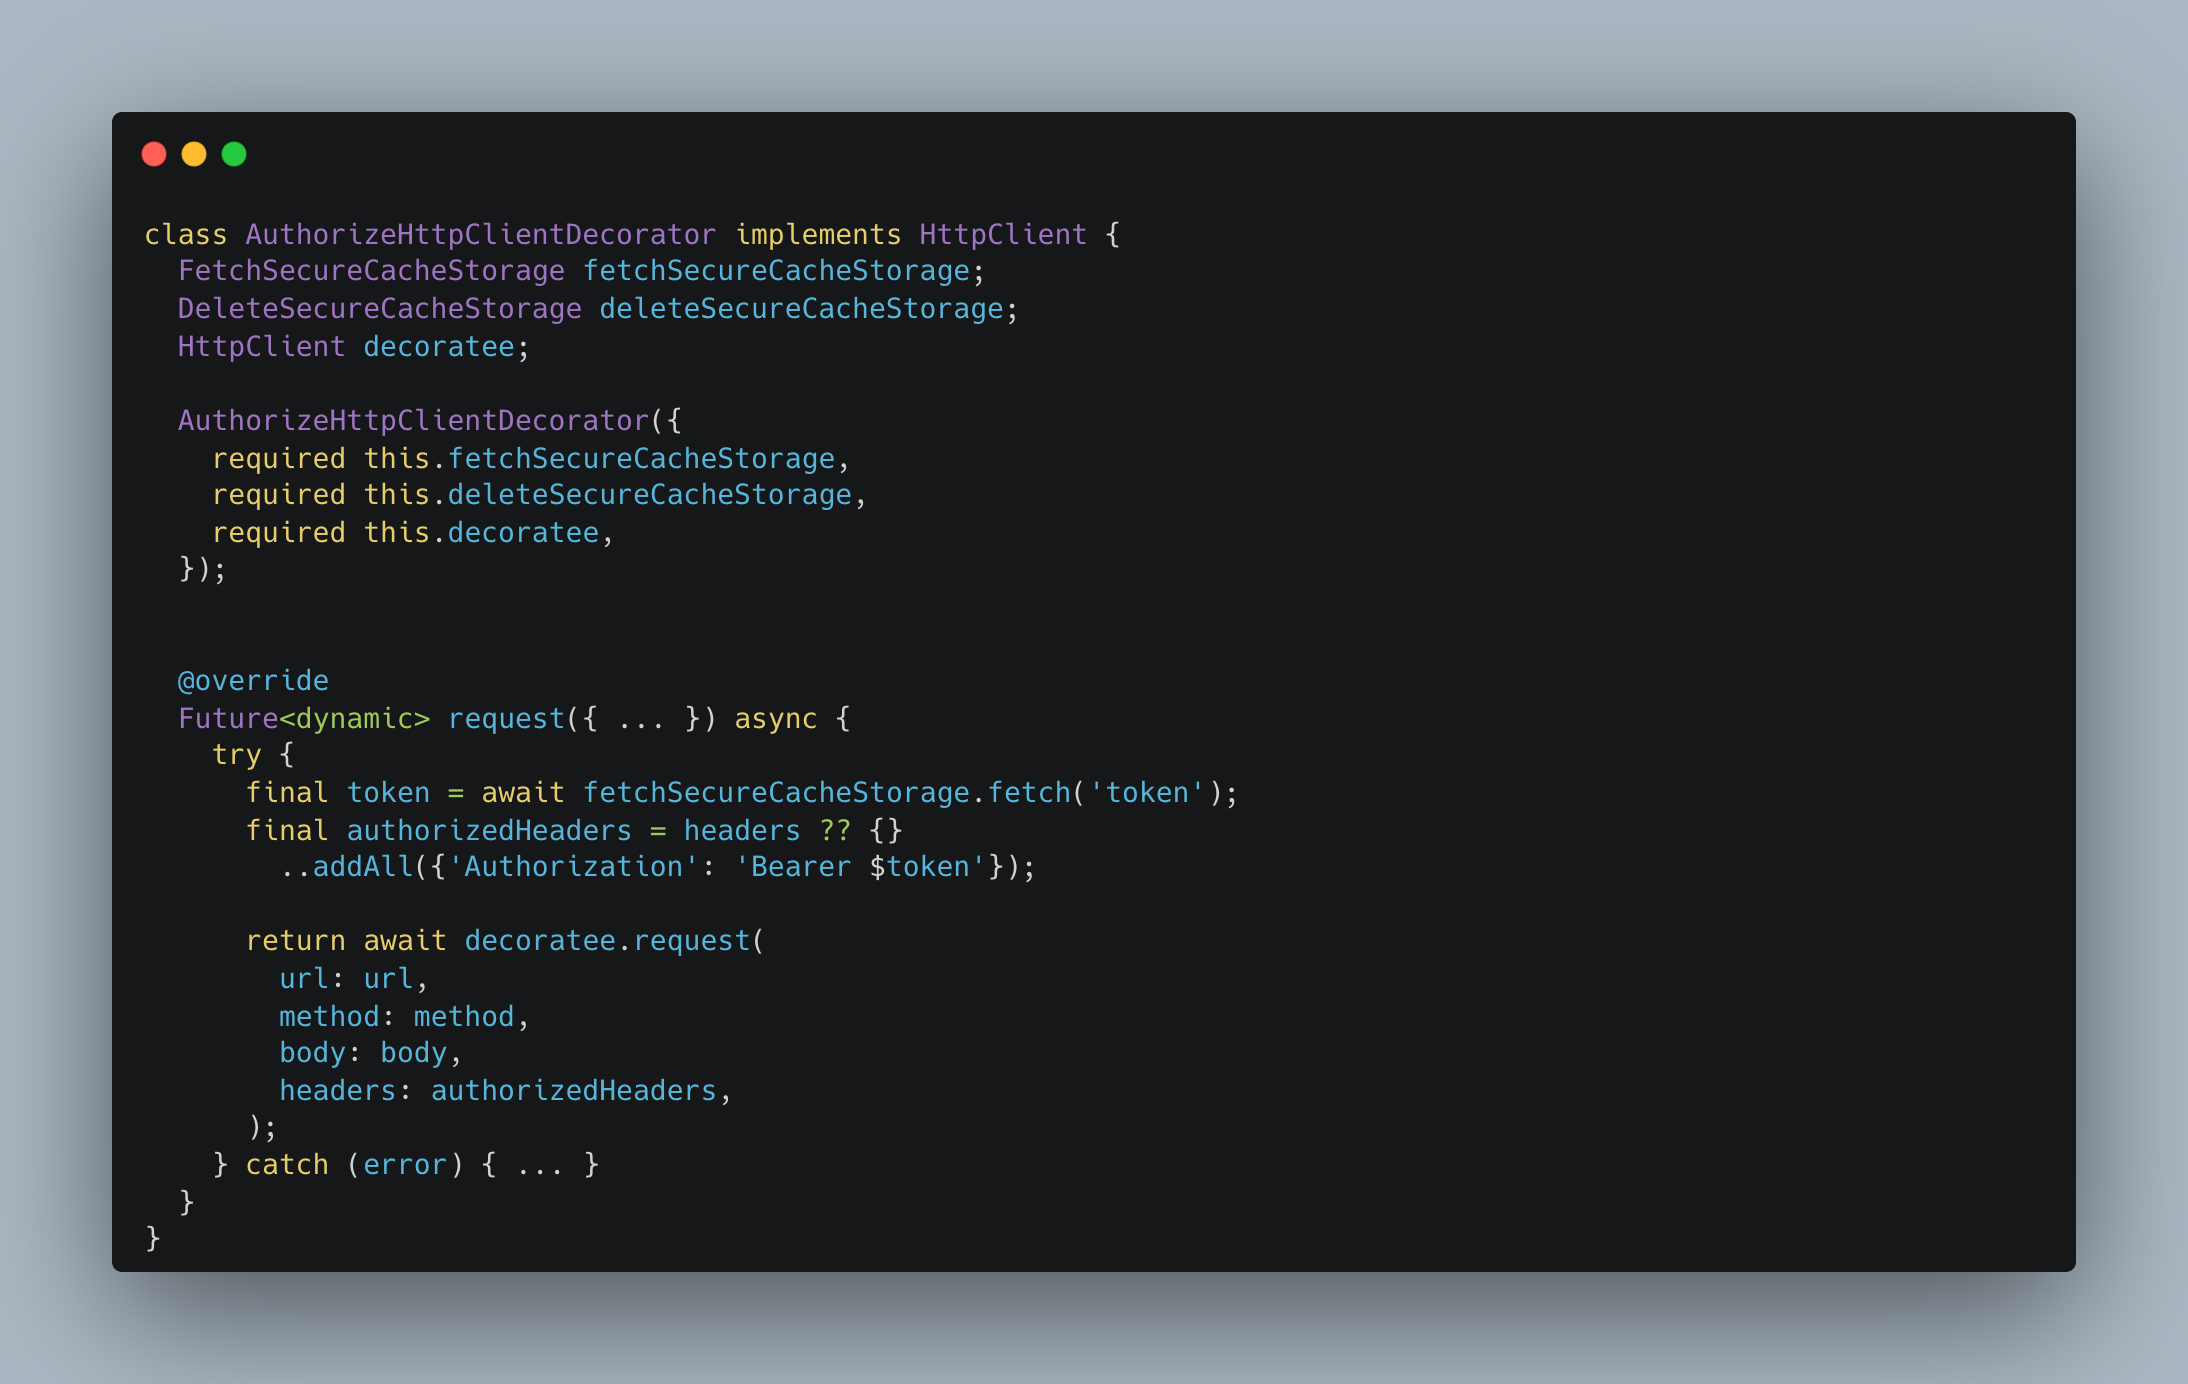
\includegraphics[width=\linewidth]{projeto/images/LSP.png}
  \caption{Liskov Substitution Principle}
  \label{fig:lsp}
\end{figure}

\subsection{Princípio da Segregação da Interface}
Neste projeto uma aplicação deste princípio é o módulo SecureStorageAdapter \autoref{fig:SecureStorageAdapter}, que é responsável pela comunicação com a memória cache dos dispositivos. Como é possível salvar, ler e deletar os dados da memória cache, foi feita a segração das ações três interfaces \autoref{fig:SecureStorageInterfaces}, dessa forma caso os dados precissasem serem obtidos de outro local, seria realizado a modificação apenas dentro do código da implementação da interface.

\begin{figure}[!ht]
  \centering
  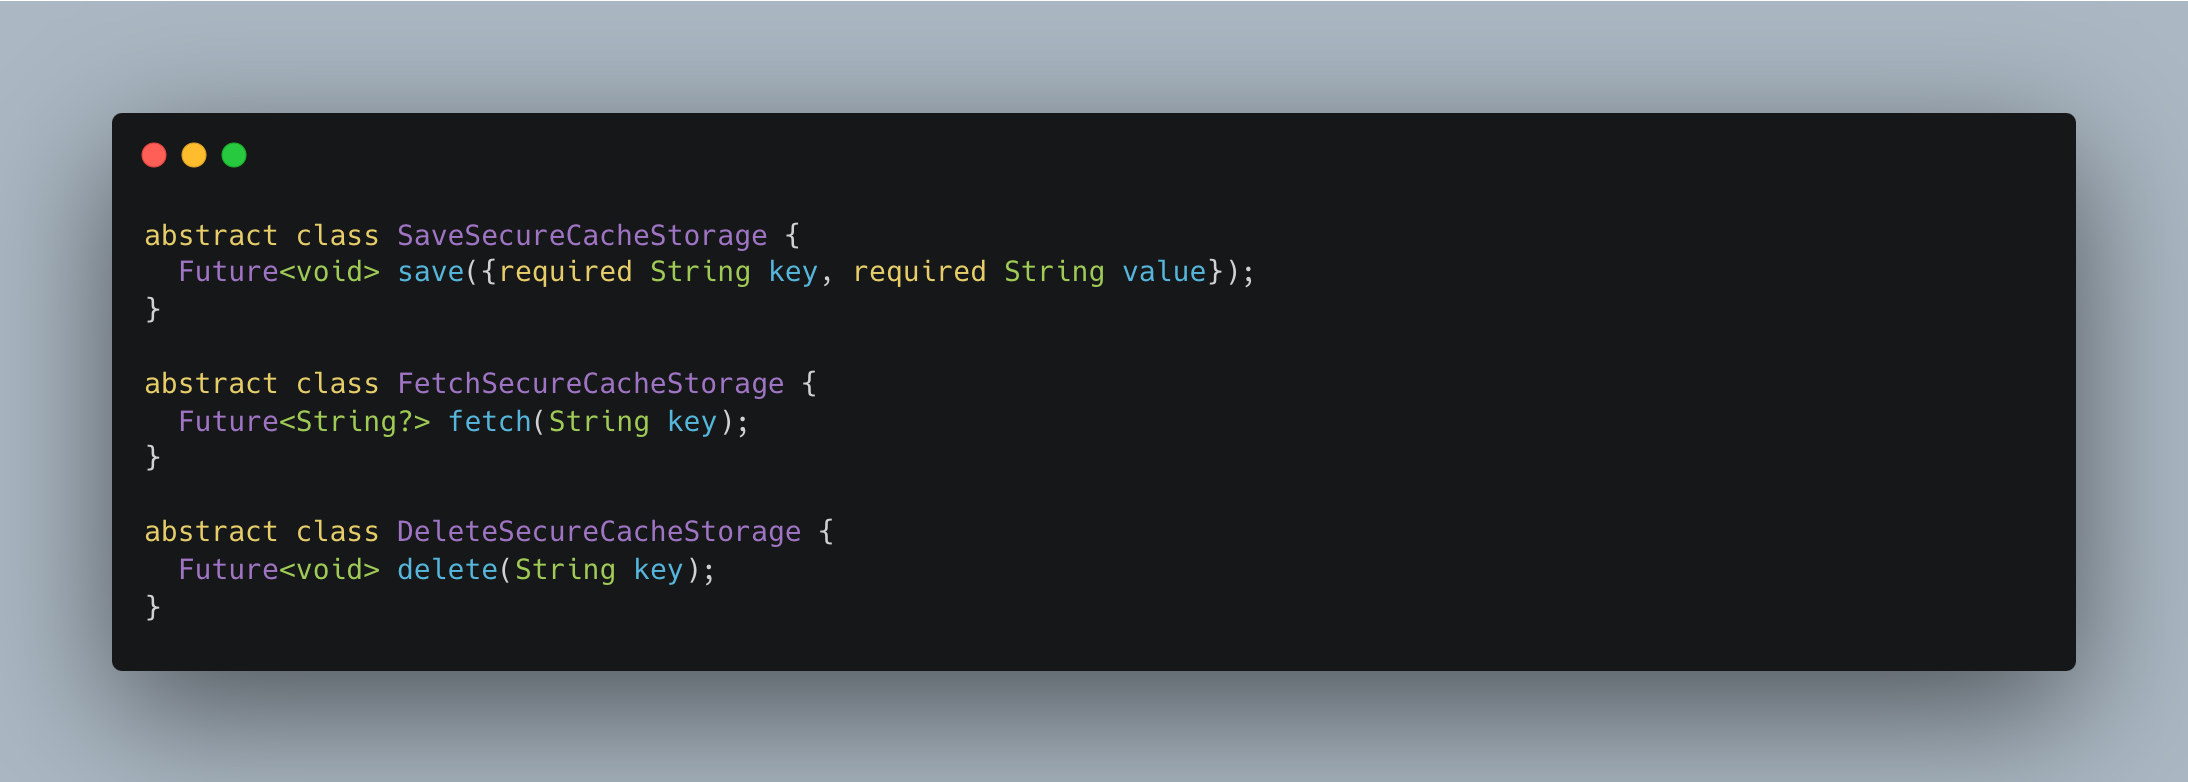
\includegraphics[width=\linewidth]{projeto/images/secure_storage.png}
  \caption{Interfaces SecureStorage}
  \label{fig:SecureStorageInterfaces}
\end{figure}

\begin{figure}[!ht]
  \centering
  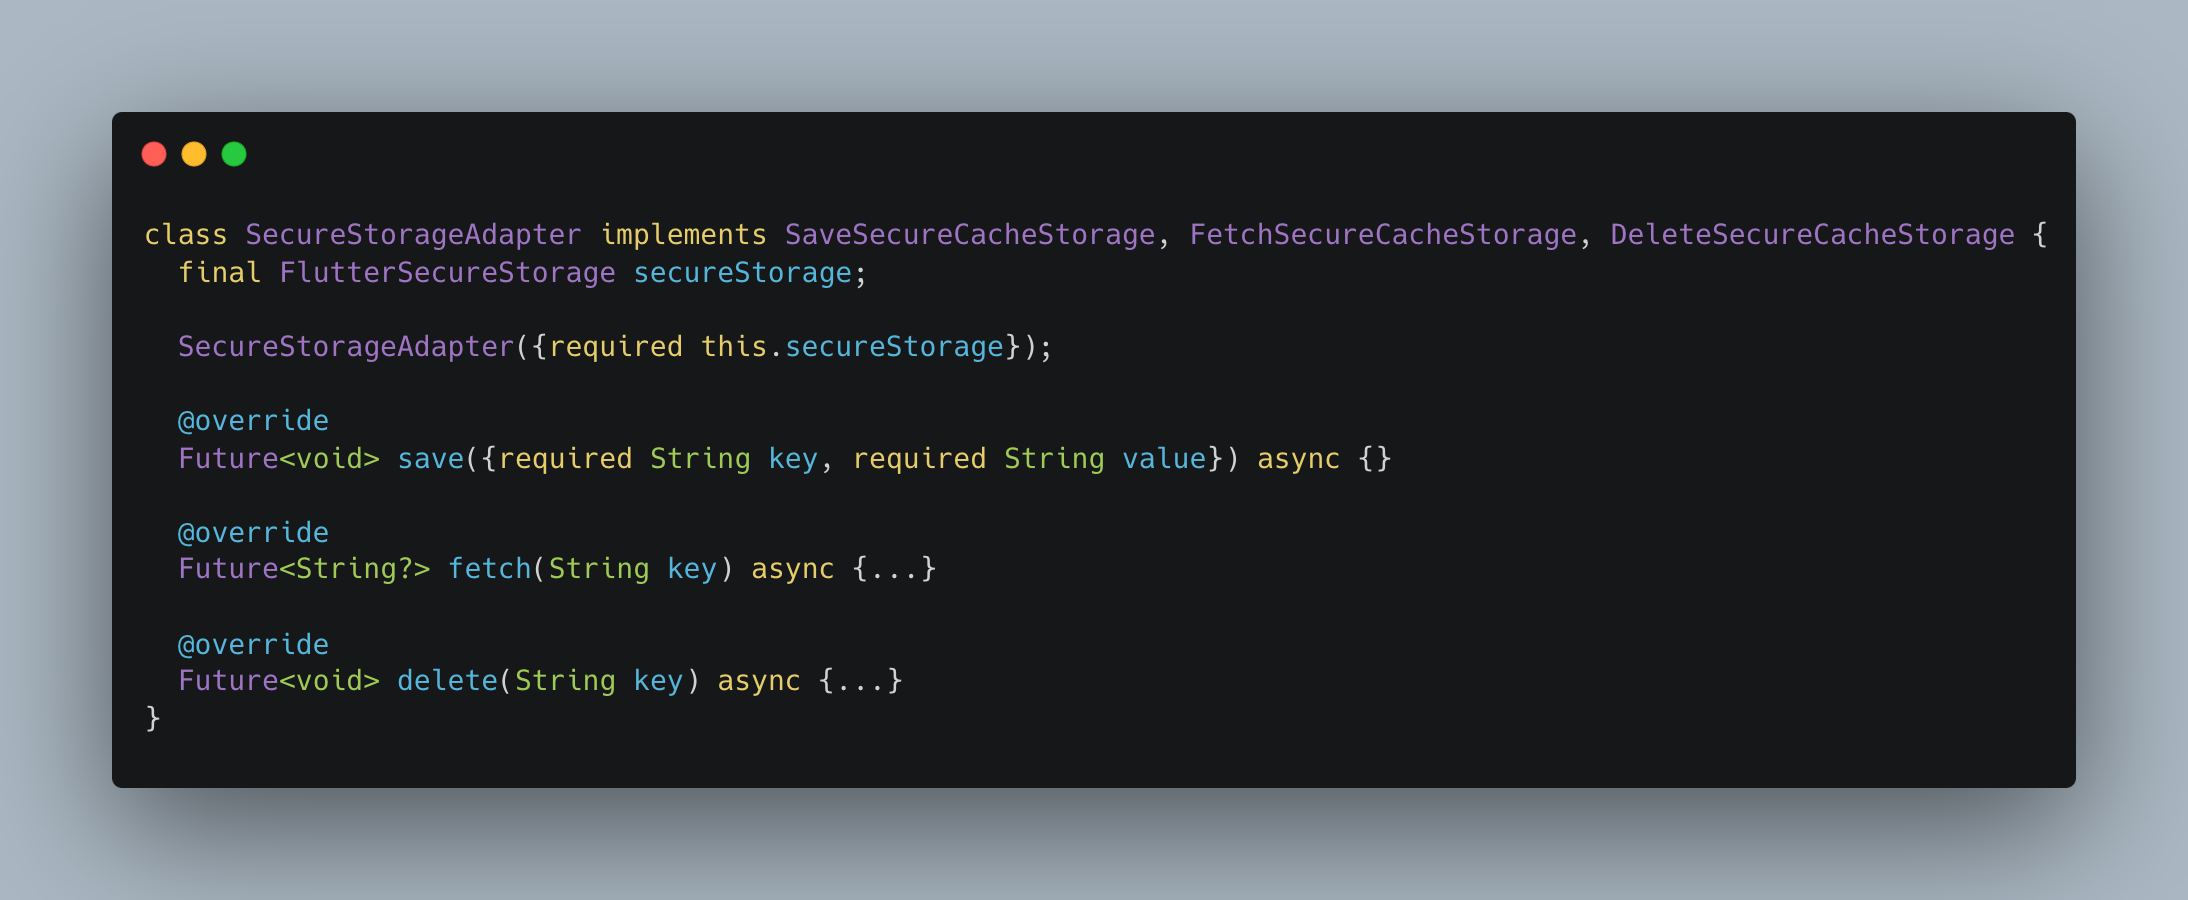
\includegraphics[width=1\linewidth]{projeto/images/secure_storage_adapter.png}
  \caption{Implementação SecureStorageAdapter}
  \label{fig:SecureStorageAdapter}
\end{figure}

\subsection{Princípio da Inversão da Dependência}
Neste projeto uma aplicação deste princípio é o caso de uso AddAccount, onde é realizada a injenção da classe abstrata HttpClient \autoref{fig:DIPHttpClient} e não da classe concreta HttpAdapter responsável por realizar as requisições Http \autoref{fig:httpClientInterface}.

\begin{figure}[ht]
  \centering
  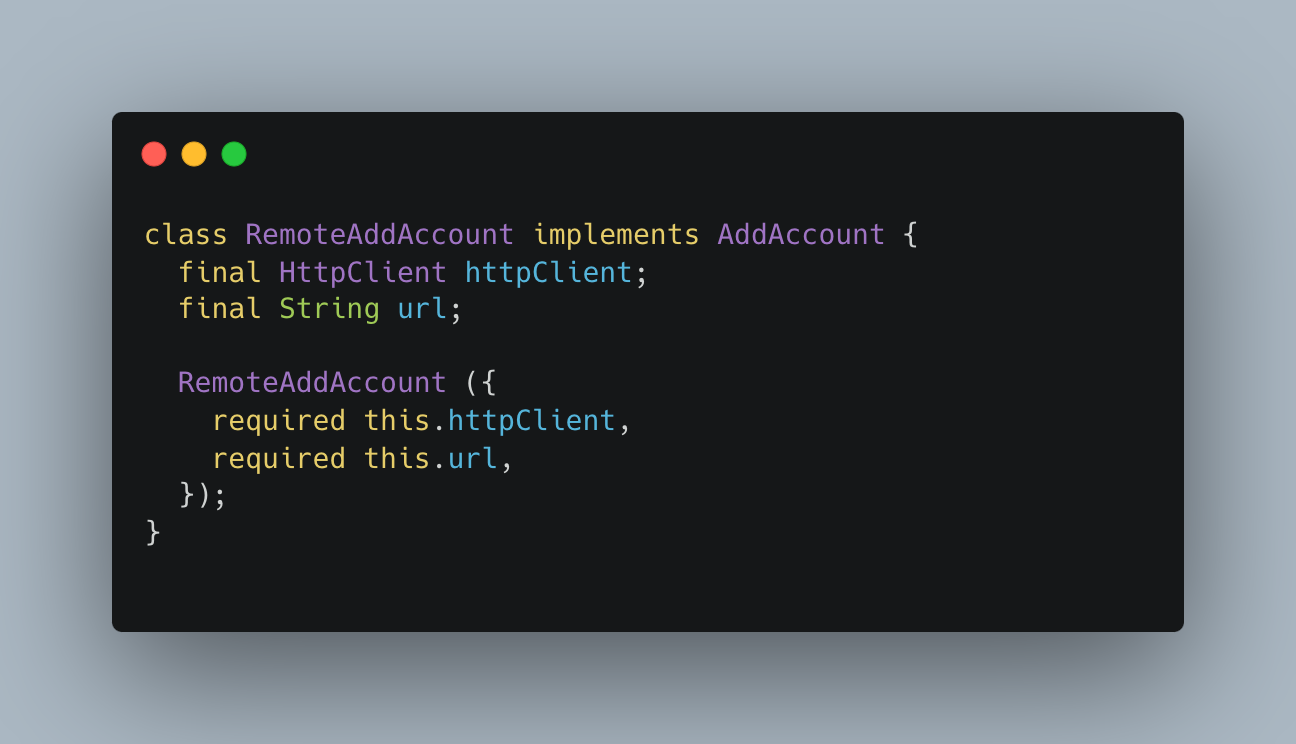
\includegraphics[width=0.7\columnwidth]{projeto/images/remote-add-addcount.png}
  \caption{Injenção da dependência HttpClient}
  \label{fig:DIPHttpClient}
\end{figure}

\begin{figure}[ht]
  \centering
  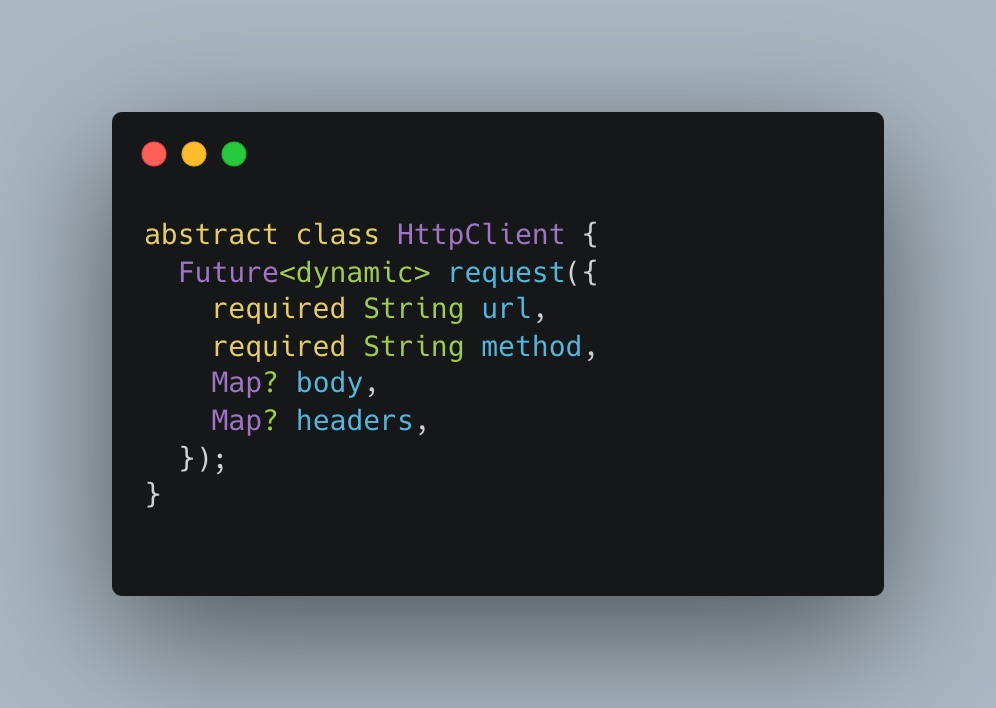
\includegraphics[width=0.7\columnwidth]{projeto/images/http-client.png}
  \caption{Interface para o módulo de requisições Http}
  \label{fig:httpClientInterface}
\end{figure}

\section{Test Driven Development}
\label{apx:tdd}
Aplicando a prática do TDD para desenvolver este projeto foi possível obter uma cobertura de testes de cerca de 85.1\%, como mostra a Figura \ref{fig:testeCoverage}. Conforme as melhores práticas de cobertura de código da Google, \cite{codeCoverage} a cobertura de testes do projeto ficou na faixa "Recomendável", que fica entre 75\% a 90\%. Por outro lado, as camadas que possuem regras de negócios (data, domain, infra, validation) tiveram uma cobertura de testes de 100\%.

\begin{figure}[ht]
  \centering
  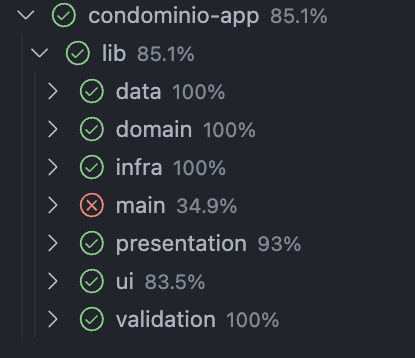
\includegraphics[width=0.5\linewidth]{projeto/images/TesteCoverege.png}
  \caption{Cobertura de Testes}
  \label{fig:testeCoverage}
\end{figure}

\end{appendices}

\end{document}
